\documentclass[acmsmall,review,anonymous]{acmart}\settopmatter{printfolios=true,printccs=false,printacmref=false}

\usepackage{times}
\usepackage{datetime}
\usepackage{balance}  % to better equalize the last page
\usepackage{graphics} % for EPS, load graphicx instead
%\usepackage[T1]{fontenc}
\usepackage{url}
\usepackage{hyperref}
\usepackage{txfonts}
\usepackage{pslatex}    
\usepackage{pifont}
%\usepackage{bbding}
\usepackage{multirow}
\usepackage{makecell}
\usepackage[justification=centering]{caption}
\usepackage{xspace}
\usepackage{comment}
\usepackage{listings}
%\usepackage[section]{placeins}
\usepackage{tikz}
\usepackage{calc}
\usepackage{fancyvrb}
\usepackage{xcolor}
\usepackage{flushend}
\usepackage{wrapfig}

\newcommand{\cmark}{\ding{51}}%
\newcommand{\xmark}{\ding{55}}%

\newcommand{\eurosyssubmissionnumber}{\#147, 12 pages}
\newcommand{\todo}[1]{{\color{red}\bfseries [[#1]]}}
\newcommand{\TP}[1]{{\color{red}\bfseries [[#1]]}}

\newcommand{\Watcher}{{Watcher}}
\newcommand{\WA}{{Watcher}}
\newcommand{\ASAN}{{ASan}}
\newcommand{\DT}{{DoubleTake}}

\newcommand{\OB}{\texttt{OpenBSD}}
\newcommand{\DieHarder}{\texttt{DieHarder}}
\newcommand{\DL}{\texttt{DLmalloc}}
\newcommand{\JE}{\texttt{jemalloc}}
\newcommand{\NA}{\texttt{numalloc}}
\newcommand{\NM}{\texttt{numalloc}}


\newcommand{\pthread}{\texttt{pthread}}
\newcommand{\pthreads}{\texttt{pthreads}}
\newcommand{\specialcell}[2][c]{%
  \begin{tabular}[#1]{@{}c@{}}#2\end{tabular}}

%%
%% \BibTeX command to typeset BibTeX logo in the docs
\AtBeginDocument{%
  \providecommand\BibTeX{{%
    \normalfont B\kern-0.5em{\scshape i\kern-0.25em b}\kern-0.8em\TeX}}}


% May send this work to Emery and Qiang zheng for their feedbacks. 

\begin{document}

\title{NUMALLOC: Adaptive NUMA Memory Allocator}
\author{Anonymous}

The NUMA architecture accommodates the hardware trend of an increasing number of CPU cores. It requires the cooperation of memory allocators to achieve good performance for multithreaded applications. Unfortunately, existing allocators \NEW{do not} support NUMA architecture well.
% \todo{Unfortunately, none of the existing allocators can support NUMA architecture well}.
This paper presents a novel memory allocator -- \NM{}, that is designed for the NUMA architecture. \NM{} is centered on a binding-based memory management. On top of it, \NM{} proposes an ``origin-aware memory management'' to ensure the locality of memory allocations and deallocations, as well as a method called ``incremental sharing'' to balance the performance benefits and memory overhead of using transparent huge pages.
% On top of it, \NM{} proposes a method called ``incremental sharing'' to balance the performance benefits and memory overhead of using transparent huge pages, as well as an ``origin-aware memory management'' to ensure the locality of memory allocations and deallocations. 
% It further introduced an interleaved heap to reduce the load imbalance among different nodes and an efficient mechanism for object movement.
% It further introduced origin-aware memory management to ensure the locality of memory allocations and an interleaved heap to reduce the load imbalance among different nodes. 
% Evaluation results show that 
According to our extensive evaluation, \NM{} has the best performance among all evaluated allocators, running \NEW{15.7\%} faster than the second-best allocator (mimalloc), and \NEW{19.0\%} faster than the default Linux allocator with reasonable memory overhead. 
% For the best case, \NM{} achieves up to $6.8\times$ performance speedup compared to other allocators. 
\NM{} is also scalable to 128 threads and is ready for deployment.

\maketitle


\date{}

\keywords{Non-Uniform Memory Access, Memory Allocator, NUMA Allocator}  %% \keywords are mandatory in final camera-ready submission


\section{Introduction}
\label{sec:intro}

The Non-Uniform Memory Access (NUMA) architecture is an appealing solution for the scalability of multi-core era. Compared to Uniform Memory Access (UMA) architecture, the NUMA architecture avoids the bottleneck of a central memory controller: each processor (also known as a domain or node) consists of multiple cores, while each node can access its own memory controller. Different nodes are connected via high-speed inter-connection (such as Quick Path Interconnect (QPI)~\cite{intelqpi} or HyperTransport bus~\cite{hypertransport}) to form a cache-coherent system that presents an abstraction of a single globally addressable memory. 
However, NUMA applications may have serious performance issues, if programs have one of the following issues, such as large amount of remote accesses, load imbalance, contention for interconnection, memory controller, and last level cache~\cite{Blagodurov:2011:CNC:2002181.2002182, Dashti:2013:TMH:2451116.2451157}, as discussed more in Section~\ref{sec:overview}. 

Multiple types of approaches help improve the performance of NUMA systems. The first type of approaches migrates tasks or physical pages reactively based on memory access patterns or other hardware characteristics~\cite{Blagodurov:2011:CNC:2002181.2002182, AutoNUMA, Dashti:2013:TMH:2451116.2451157, Lepers:2015:TMP:2813767.2813788}. They improve the performance automatically without human involvement. However, these systems impose additional overhead (sometimes unnecessarily)  by migrating tasks or physical pages reactively. Further, the migration cannot reduce remote accesses if objects of the same page are concurrently accessed by  threads in multiple nodes~\cite{Gaud:2014:LPM:2643634.2643659}. 
The second type of approaches relies on programmers to manage memory allocations and task assignments explicitly~\cite{Kaestle:2015:SSA:2813767.2813787, Lin:2016:MTP:2872362.2872401, Majo:2017:LPC:3057718.3040222}. Although they could improve the performance greatly, they typically require significant human effort to rewrite the programs, where legacy systems cannot benefit automatically. 

Another type of approach focuses on heap management~\cite{tcmallocnew, kim2013node, yang2019jarena}. The NUMA-aware memory management is appealing, because there is no need to change applications explicitly. Also, they are belonging to proactive approaches that could reduce remote accesses without task or page migration. Among them, Kaminski et al. designs the first NUNA-aware memory allocator~\cite{tcmallocnew}, called as TcMalloc-NUMA in the remainder of this paper, where the other two papers utilize a similar approach. TcMalloc-NUMA invokes the \texttt{mbind} system call to bind the memory explicitly to the node that a thread is running on, and guarantees local allocation initially.  
%Due to the explicit binding, it is able to check the locality of a memory block inside the user space, and then return a freed object back to the corresponding node based on the locality. TcMalloc-NUMA achieves some performance speedup for some synthetic applications. 

However, TcMalloc-NUMA has load imbalance issue and locality issue as follows. First, it always allocates the memory from the node that the thread is currently running on. But it may cause significant performance issue if a thread is migrating to a new node, since a thread is forced to access its remote stack, and will lose the locality of cache lines. Further, this design is not tapped with the OS scheduler. As observed by previous study~\cite{Grace}, the OS scheduler typically assigns newly-created threads into the same processor as the parent thread in order to exploit cache locality. However, all pages allocated in the original node will be remote accesses, if a thread is dispatched to a remote node afterwards.  Second, it does not consider the load balance issue.  All objects that allocated in the main thread but accessed concurrently by multiple children threads will be located in the same node, causing the load imbalance issue. Third, it does not employ the recent progress of the hardware and OS support, such as huge page support. Fourth, its memory management cannot ensure the locality, if an object is deallocated by a thread that is different from the allocating thread. For such objects, \TN{} will simply place them into the local cache of the current thread, generating unnecessary remote accesses.  


\begin{comment}

It first assumes that a memory block is belong to the same node for its allocating thread. However, this assumption is invalid, and is also contradict with the first-touch policy of the OS. 

If there is no such assumption, we will expect that the OS will provide an efficient API to query the locality of a page. However, no such APIs exist in both Linux and Windows. 

It checks the physical memory usage to determine the future allocations of the same node or the re-use of a remote node. But that is very slow by checking meminfo. 

In the end, it utilizes the mbind to bind the memory to a node specifically. 
	
\end{comment}
	 

%Based on our evaluation, TcMalloc-NUMA cannot achieve good performance for many applications.  
%However, none of these systems could achieve the performance promised by the hardware. Given a simple example, if one page is fulled with objects that are utilized by different threads running on different nodes, then it is not able to achieve the best performance no matter where this page is located. Similarly, the passive tracking of memory ownership of an object cannot completely avoid the ownership drifting problem, where the . 

This paper proposes a novel NUMA-aware memory allocator -- \NM{} -- to address these  issues. \NM{} improves both load balance and locality with the following designs.  

First, \NM{} proposes a \textbf{binding-based memory management policy} that ensures both load balance and locality. For load balance, \NM{} binds threads to different NUMA nodes in an interleaved way. That is, a newly -created thread will be always bound to a different node from its predecessor. Because of this binding policy, every node will have a similar number of threads, ensuring load balance between different memory controllers. Due to the binding, a thread will not be migrated to a different node, avoiding the performance loss caused by cross-node thread migration. For the locality, \NM{} reserves a range of virtual memory for each node, where all physical pages can be only allocated from this node (specified via \texttt{mbind} system call). For each thread, allocations can be only satisfied from its per-node heap, or from a per-thread cache that always tracked freed objects originated from the same node. More specifically, \NM{} checks the node locality of an object upon the deallocation, and only places an object into its per-thread cache if it is originated from the same node. Otherwise, the object will be returned to its original node. This is different from \TN{}. \NM{} also reduces locality issues by always allocating the metadata from the local node.  


% task management altogether, by binding tasks to different NUMA nodes interleavedly and binding the memory explicitly. The task binding not only benefits the load balance, due to its even distribution of tasks, but also constructs the basis for its memory management. In this design, there is no need to query the locality of tasks dynamically, and it is guaranteed to have the correct locality for the memory. 
  
Second, \NM{} further proposes \textbf{an interleaved heap} to reduce the load imbalance issue. More specifically, \NM{} reserves a range of virtual memory that physical pages will be allocated interleavedly across all physical nodes. That is, physical pages from the interleaved heap will be evenly allocated from all nodes, avoiding the congestion of one memory controller~\cite{Blagodurov:2011:CNC:2002181.2002182}. However, a naive method of allocating all objects from the interleaved heap may actually cause unnecessary remote accesses. For instance, private objects should be always allocated in the local node, instead of from the interleaved heap. \NM{} only allocates potentially-shared objects from the interleaved heap, and proposes a heuristics method to determine such objects, as described in Section~\ref{sec:mainthread}.  

 Third, \NM{} proposes new huge page support, by employing the recent progress of the hardware and the OS. Note that this is different from the default support of transparent huge page. As observed by existing study~\cite{Gaud:2014:LPM:2643634.2643659, DBLP:conf/asplos/PanwarBG19}, the transparent huge page mechanism has a harmful impact on the performance for the NUMA architecture, due to memory waste and page-level false sharing. Differently, \NM{} only utilizes huge pages for big objects and small objects that are allocated extensively. \NM{}'s huge page support minimizes both memory waste and page-level false sharing. Based on our evaluation, \NM{}'s huge page support is always benefiting the performance (Section~\ref{sec:hugepage}). 
 
 Besides that, \NM{} is implemented very carefully in order to achieve the good performance. It introduces many implementation techniques, such as fast metadata lookup, cache warmup mechanism, efficient objects migration, node-local metadata, as further described in Section~\ref{sec:implement}. 
 
% Second, it proactively bound the memory to different nodes, so that it could reduce the . Third, it takes a different method to deal with allocations from main thread, Fourth, it takes the advantage of hardware progress automatically, e.g., huge pages. One application achieves 10\% performance speedup with this consideration.  


%There are other implementation issues that may also contribute to the performance improvement. For instance, the metadata will be always allocated locally. The big objects will be re-utilized by small objects automatically, in order to reduce the potential cache misses. 

We have performed extensive evaluation on synthetic and real applications, and compared \NM{} with popular allocators, such as the default Linux allocator, TcMalloc~\cite{tcmalloc}, jemalloc~\cite{jemalloc}, Intel TBB~\cite{tbb}, and Scalloc~\cite{Scalloc}. For the performance on real applications, \NM{} achieves around 13\% speedup on average comparing to the default Linux allocator, which is also 11\% faster than the second best one. For the best case, \NM{} achieves up to $5.8\times$ faster than the default allocator, and $4.7\times$ faster than the second best one (TcMalloc). For four synthetic applications, \NM{} is running around $2.2\times$ faster on average than the second best one on an 8-node machine. In total, \NM{} may impose around 23\% memory overhead, but is much more scalable than all other allocators.  \NM{} is ready for the practical employment, due to its high performance, and good scalability. 

Overall, this paper has the following contributions. 

\begin{itemize}
\item \NM{} proposes a binding-based memory management that integrates task management with memory management together. This design ensures both load balance and locality.  
\item \NM{} proposes an interleaved heap in order to reduce load imbalance issue caused by shared objects. 
\item \NM{} proposes new huge page support that  minimizes memory waste and avoids page-level false sharing, which always benefits the performance. 
\item \NM{} includes multiple careful designs to reduce the performance and memory overhead, such as fast metadata lookup, efficient objects migration. 
\item The extensive experiments confirm that \NM{} has a better performance and scalability than even widely-used industrial allocators. 
\end{itemize}

The remainder of this paper is organized as follows. Section~\ref{sec:overview} introduces the NUMA architecture and the corresponding OS support. Section~\ref{sec:implement} focuses on the design and implementation of \NM{}. After that, Section~\ref{sec:evaluation} describes its experimentation evaluation, and Section~\ref{sec:limit} discusses the limitation of \NM{}. In the end, Section\ref{sec:related} discusses some relevant related work, and then Section~\ref{sec:conclusion} concludes. 

\begin{comment}

eve have evaluated it on a range of benchmarks and real applications on two different NUMA architecture. The evaluation showed that \NA{} could significant improve the performance by up to 2X, with the average of 10\% performance. The evaluation also show that \NA{} has a bigger performance improvement on  


 
How to design the new allocator? This is the new one. 

We will try to achieve the following target. 

(1) The performance will be as efficient as possible. 
(2) It is still 
For information-computable, we will achieve the following targets:
We should still use the address to infer the following information, such as the size of the object and the shadow memory placement.

We don't support many bags for the same size class, just one big bag for each size class of each heap. Why it is necessary? 

We would like to reduce the memory blowup as much as possible, where the memory will be returned back to the current thread's heap. 

In order to support that, maybe we could have a big heap for the same size class, but different threads will start from different placement. 

Is it good for the NUMA support in the future? For NUMA support, it is great if we can always return the memory back to its original 


Virtual address will be divided into multiple nodes. 

Then inside each step, we will divide a sub-heap into multiple mini-heaps, where each mini-heap will support one thread. 


Virtual address will be divided into multiple nodes. 

Then inside each per-node heap, we will further divide it into multiple mini-heaps, where each mini-heap will support one thread in order to reduce the possible contention. 

For each per-thread heap, we will have two free-lists for each size class. The first one will be used for the current thread, without the use of lock at all. The second one will be utilized for returning memory from other threads.  

RTDSCP is a way to know where a thread is executed on. 

%https://software.intel.com/en-us/forums/intel-isa-extensions/topic/280440

Should we put the metadata into the corresponding node? We will minimize the lock uses for each node, since that will invoke unnecessary remote accesses as well. 


% From Score: SCOREs runtime system will include a memory manager instrumented to track object ownership with low overhead by leveraging existing thread-local allocation buffers and using per-processor memory pools. The runtime system will sample memory access patterns to detect when memory should be relocated to or initially placed in memory closer to a specific processor

What is the uniqueness of NUMA architecture? 

Remote accesses and imbalance? 
What are the big issues that could cause the performance issues on the NUMA architecture. 

Programs also have some inherent imbalance. For instance, main thread typically will prepare the data for all children threads. Therefore, many existing tools discover that the block-wised allocation is one way to reduce the imbalance~\cite{XuNuma, XXX}. 
Also, many applications are typically utilizes a producer-consumer architecture, where the objects allocated in one thread will be deallocated by another thread. This issue, if not handle correctly, will cause the ownership thrifting issues, which will cause that it is impossible to know the placement of an object after a while. Very quickly, it may cause a lot of unnecessary remote accesses, when using the existing NUMA allocator~\cite{}.  

Therefore, a good NUMA allocator should deal with these inherent imbalance of programs. Also, it should deal with the normal problems of NUMA hardware. It should 
	
\subsection{Novelty}

\begin{itemize}
\item We will design a node-aware memory allocator that could actually identify the memory placement by using the virtual address.
\item We will minimize the synchronization, since that will impose unnecessary remote accesses. 
\item We will minimize remote accesses by putting the metadata into multiple nodes. 
\item We may support multiple types of allocation, such as block-wise false sharing memory accesses, or node-balanced memory accesses, relying on the indication from user space. 	
\item We will balance the memory consumption over all nodes, in order to avoid the contention of memory controller~\cite{Majo:2011:MSP:1987816.1987832}.  At least, we could balance the memory consumption among all allocators. Ideally, it is better to balance the memory accesses. 
\item We may track the relationship of all objects. Then those objects will be allocated correspondingly. For instance, if the objects are allocated in the main thread, we assume that they will be accessed as a shared mode. Then we would like to allocate in the node-balanced areana initially. 

\end{itemize}

\end{comment}


\begin{comment}


\begin{enumerate}
\item Dividing each node's memory into two parts, one for small objects, and one for big objects. 
\item Making the main thread to use a dedicate memory region. Memory will be allocated in different nodes in an interleaved way. However, this method has some benefits and shortcomings. If the memory is deallocated immediately, then it is time-consuming to put it remotely, and will hurt the performance. Therefore, it is necessary to identify such cases, and do not allocate such objects in the interleaved way. 
\item Fixing the merge and split for big objects
\item Thinking about the integration of Ding Chen's theory. (Let Xin to do this part)
\item Thinking about using the inside of the object for holding the pointers for link list, which will be faster and remove some memory overhead unnecessarily. (Let Xin to do this part)
\item For producer-consumer threads, we will also track which objects are allocated and freed in different threads. For those objects, maybe they could utilize the same mechanism as the main thread. But we will do this in the future.
%\item Could we use page-spans instead to ensure the sharing? 
\item Intercepting mmap and use the mainthread's interleaved idea. 

\item We will use huge pages by default in order to improve the performance. But we will utilize small bags for small size classes, which we will learn from TcMalloc. That is, we don't want to use 1 Megabyte information. Instead, we may utilize the 4 pages as an unit. 

	
\end{enumerate}
	
\end{comment}


\section{Background}
\label{sec:background}

%This section introduces some background that is necessary for \NM{}. 
This section discusses the NUMA architecture, existing OS support and common design of memory allocators.
%for the NUMA architecture, and then discusses some common designs of existing memory allocators that are adopted by \NM{}.  

\subsection{NUMA Architecture}

\label{sec:numa}

%Traditional computers are using the Uniform Memory Access (UMA) model that all CPU cores are sharing a single memory controller, where any core can access the memory with the same latency (uniformly). However, the UMA architecture cannot accommodate the hardware trend with the increasing number of cores, since all cores may compete for the same memory controller. 
%Therefore, the performance bottleneck is the memory controller in many-core machines, since 
%A task cannot proceed without getting its necessary data from the memory. 

The Non-Uniform Memory Access (NUMA) architecture is to solve the scalability issue, due to its decentralized nature. Instead of making all cores waiting for the same memory controller, the NUMA architecture typically is installed with multiple memory controllers, where a group of CPU cores has its memory controller (called a node). Due to multiple memory controllers, the contention for the memory controller could be largely reduced and therefore the scalability could be improved correspondingly. However, the NUMA architecture also has multiple sources of performance degradations~\cite{Blagodurov:2011:CNC:2002181.2002182}, including \textit{Cache Contention}, \textit{Node Imbalance}, \textit{Interconnect Congestion}, and \textit{Remote Accesses}.  

%\textit{Cache Contention:} the NUMA architecture is prone to cache contention that multiple tasks may compete for the shared cache. Cache contention will introduce more serious performance issue if the data has to be loaded from a remote node. 
 
%\textit{Node Imbalance:} When some memory controllers have much more memory accesses than others, it may cause the node imbalance issue. Therefore, some tasks may wait more time for memory accesses, thwarting the whole progress of a multithreaded application.  

%\textit{Interconnect Congestion:} Interconnect congestion occurs if some tasks are placed in remote nodes that may use the inter-node interconnection to access their memory. 

%\textit{Remote Accesses:} In NUMA architecture, local nodes can be accessed with less latency than remote accesses. Therefore, it is important to reduce remote accesses to improve the performance.\\


Based on the study~\cite{Blagodurov:2011:CNC:2002181.2002182}, node imbalance and interconnect congestion may have a larger performance impact than cache contention and remote accesses. These performance issues cannot be solved by the hardware automatically. Software support is required to control the placement of tasks, physical pages, and objects to achieve the optimal performance for multithreaded applications.  

\subsection{NUMA Support Inside OS} 

Operating System already supports the NUMA architecture, especially on task scheduling and physical memory allocation. For task scheduling support, the OS provides some system calls that allow users to bind a task to a specific node. For memory allocation, the OS provides system calls (e.g., \texttt{mbind}) to change memory allocation policy for a range of memory or for the whole process~\cite{lameter2013numa, diener2015locality}. However, those system calls still require programmers to specify the policy explicitly, which cannot, therefore, automatically provide the performance improvements. \NM{} relies on these existing system calls to manage memory allocations explicitly, as further described in Section~\ref{sec:implement}, but without changing the user program explicitly. Linux also supports Automatic NUMA balancing (AutoNUMA)~\cite{AutoNUMA1}, which migrates the tasks closer to the memory they are accessing. 

\subsection{Common Designs of Memory Allocators}
\label{sec:commondesign}

Memory allocators share some common designs. First, most allocators manage objects differently based on the size of objects. For big objects, allocators may request objects from the OS directly and return them to the OS directly upon deallocation~\cite{Hoard}. On the other hand, small objects will be tracked in freelists based on size classes. Managing small objects can be further classified into multiple categories, such as sequential and BiBOP, where region-based allocators do not belong to general-purpose allocators~\cite{DieHarder, Gay:1998:MME:277650.277748}. 
%For region-based allocators, all objects within the same region are deallocated together~\cite{Gay:1998:MME:277650.277748}.  But region-based allocators do not belong to general-purpose allocators. 
For sequential allocators, subsequent memory allocations are satisfied in a continuous memory block~\cite{Cling}. BiBOP-style allocators, which stands for ''Big Bag of Pages''~\cite{hanson1980portable}, utilize one or multiple continuous pages as a ``bag'' that holds objects of the same size class. 
Now many performance-oriented allocators~\cite{tcmalloc, jemalloc, Scalloc}, and most secure allocators~\cite{openbsd, DieHarder, FreeGuard, Guarder}, belong to this category. Second, to support multithreaded applications, modern allocators (e.g., TCMalloc) often implement the ``per-thread heap'' that tracks deallocated objects from the current thread~\cite{tcmallocnew}, where allocating objects from per-thread heaps do not need to acquire locks. Therefore, the per-thread heap is expected to reduce the contention between threads. A per-thread heap returns objects to a common heap shared by multiple threads, when the number of objects or the size of freed objects is larger than a threshold. \NM{} borrows these common designs in its implementation. 

%\NA{} only tracks the size information of each page, which helps reduce its memory overhead for the metadata. Third, \NA{} utilizes freelist to manage freed objects. Every freed object will be added into a corresponding freelist, and objects in the freelist will be allocated first in order to reduce possible cache misses. Further,  This mechanism helps to reduce the memory overhead, but is prone to memory vulnerabilities, such as buffer overflows and double-frees~\cite{DieHarder, Guarder}.     
 
\section{Design and Implementation}
\label{sec:implement}

\NM{} is designed as a replacement memory allocator. It intercepts all memory allocation/deallocation invocations via the preloading mechanism, and redirects them to \NM{}'s implementation. Therefore, there is no need to change the source code of applications, and there is no need to use a custom OS or hardware. In the following, we first discuss \NM{}'s basic heap layout, and then discuss multiple components that separate it from existing allocators.

\subsection{Basic Heap Layout}
\label{sec:overview}

\begin{figure}[!ht]
\begin{center}
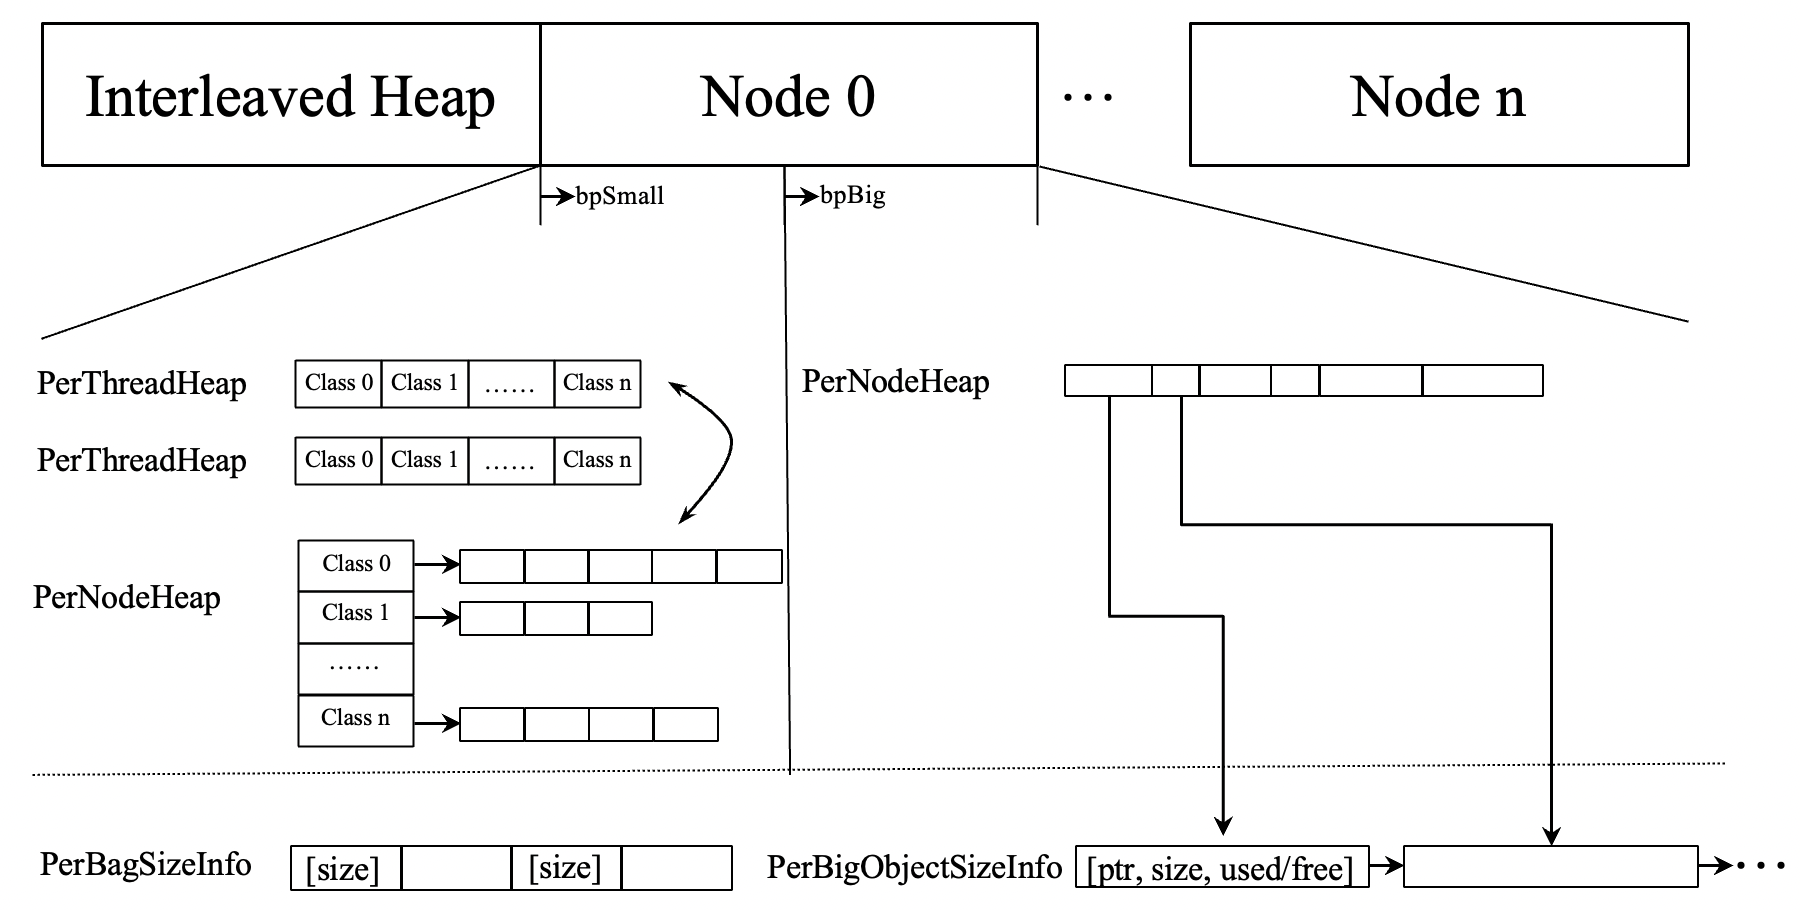
\includegraphics[width=0.45\textwidth]{SC2022/figure/numalloc-overview.png}
%\includegraphics{figure/overview2}
\end{center}
%\vspace{-0.1in}
\caption{Overview of \NA{}'s heap layout.
\label{fig:overview}}
%\vspace{-0.1in}
\end{figure}

% \todo{We should balance what to talk about in the overview, it's a little bit long and something has repeatedly described in the following}

%As discussed in Section~\ref{sec:intro}, \NM{} designs a origin-computable mechanism that could quickly check the origin of every object upon deallocation. In order to support this, 
\NM{}'s heap layout is designed as  Fig.~\ref{fig:overview}. Initially, \NM{} requests a large and continuous block of memory from the underlying OS, and then divides it evenly into multiple regions based on the number of hardware nodes. Each region is bound to a different physical node via \texttt{mbind} system call. 
%\NM{} can support the customized binding from users. If not, it typically  
In particular, the first region is bound to the first node, the second one is bound to the second node, and so on. This design enables us to compute the physical node quickly from a memory address: we could compute the index of the physical node by dividing the heap offset by the region size. 
%This layout is different from existing allocators, based on our knowledge. 
% \todo{Numalloc's reviewer said TCMalloc also use the same mechanism. I check the code and it's true that TCMalloc use the memory tag for numa partition id}
%\NM{} borrows some of these existing mechanisms. First, it uses different mechanisms to manage small and big objects. Second, small objects are also managed by size classes using the BiBOP-style. Third, similar to existing work, such as Linux and TCMalloc~\cite{tcmalloc}, \NA{} utilizes different freelists to track freed objects, and uses the first word of freed objects to link different objects. But the difference of \NM{} is further described in Section~\ref{sec:implement}.
% From Fig.~\ref{fig:overview}, we see that 
Each node's memory region will be further divided into two sub-regions, one for small objects, and the other one for big objects. The \texttt{bpSmall} pointer is utilized to track never-allocated memory
% \todo{someone doesn't understand} 
for small objects, and the \texttt{bpBig} pointer tracks the position of big objects. Similar to existing allocators, \NM{} manages small and big objects differently. 
% In \NM{}'s design, small objects are those with a size less than 512K, which are organized by size classes and each request will be satisfied from a particular size class. 
For small objects ($<$ 512KB), each request will be satisfied from a particular size class
% \NA{} utilizes fine-grained size classes, such as 16 bytes apart for objects less than 128 bytes, and 32 bytes apart for objects between 128 bytes and 256 bytes, then power-of-2 sizes afterward. 
and \NM{} utilizes the well-known ``\textbf{Bi}g-\textbf{B}ag-\textbf{o}f-\textbf{P}ages'' (BiBOP) style that all objects in the same bag (32KB by default) will have the same size class. 
Big object allocation will be satisfied in a sequential manner and their sizes are aligned to the size of one bag.

To support the NUMA architecture, a per-node heap (PerNodeHeap in Fig.~\ref{fig:overview}) is proposed that has one freelist for each size class and one common freelist for all big objects from the current node. 
%We will talk about the relationship between per-thread freelist and per-node freelist in Section~\ref{sec:origin}. 
%For small objects, freed objects of the same size class will be tracked with a freelist.
In order to reduce the contention, \NM{} adopts a per-thread heap (PerThreadHeap in Fig.~\ref{fig:overview}) that maintains a freelist for each size class, which requires no lock protection since each thread has its own per-thread heap. However, this may introduce memory blowup~\cite{Hoard} that freed objects of a per-thread heap cannot be utilized for future allocations from other threads, which will be addressed in Section~\ref{sec:others}. 
\NM{} tracks the small objects' size information in a separate area called PerBagSizeInfo, while the big objects utilize a linked list called PerBigObjectSizeInfo to store the size and availability information, which allows coalescing multiple continuous big objects into a bigger one upon deallocations.

% \NM{} tracks the size information and availability information in a separate area:  ``PerBagSizeInfo'' of Figure~\ref{fig:overview} is used for tracking the size of each size class for small objects.

%(shown as ``PerMBInfo'' of Figure~\ref{fig:overview}): it tracks the size of each size class for small objects, and the size of the big object (aligned to 1 MB) for big objects. This data structure also includes the used/free information for big objects, which allows coalescing multiple continuous big objects into a bigger object upon deallocations. To save space, \NM{} utilizes the lowest significant bit of ``PerMBInfo'' to encode the availability information.

Overall, \NM{} includes a layout that can quickly compute the physical node (with the memory binding) and a per-node heap to support node-aware allocations. This design allows it to perform incremental sharing and origin-aware memory management efficiently, as discussed in the following sections.

%mechanisms to re and one per-node freelist for each node to track big objects. \NM{} also maintains per-node freelists to track small objects based on size classes. These freelists are singly linked lists, which uses the first word of every freed object as pointers.  Small freed objects may be migrated between per-thread freelists and per-node freelists, as further described in Section~\ref{sec: others}. 
\subsection{Binding-Based Memory Management} 
\label{sec:balance}
As described in Section~\ref{sec:intro}, thread migration will cause multiple performance issues for the NUMA architecture. Therefore, \NM{} binds each thread to a node specifically to avoid thread migration across different nodes.  \NM{} currently supports two types of binding, \textbf{node-interleaved binding} and \textbf{node-saturate binding}. Node-interleaved binding binds continuous threads to different nodes in an interleaved way so that every node will have a similar number of threads. That is, the first thread will be bound to the node that it is scheduled to run by the OS, and the second thread will be bound to its next node, and so on. Instead, the node-saturate binding will bind sufficient threads to a node first before binding to a different node. For node-saturate binding, threads to be assigned will be the same as the number of hardware cores.  \NM{} will use node-interleaved binding by default, as it has a better performance based on our evaluation. But users \NEW{can} switch to the node-saturate binding by controlling the environment variable. Further, users \NEW{can} provide their customized binding via a file, which will be supported in the future. 

Note that \NM{} only binds a thread to a node, instead of a core, which still allows the scheduling initiated by the OS. To perform the binding correctly, \NM{} obtains the hardware topology in the initialization phase via the \texttt{numa\_node\_to\_cpus} API, which tells the relationship between each CPU core and each 
% memory 
node. Then it intercepts all thread creations in order to bind a newly-created thread to a specific node.

\subsection{Origin-Aware Memory Management} 
\label{sec:origin}

%\todo{In Section III-B, you talk about satisfying allocations from the "un-allocated region" as the last step. Is this memory that is not part of the interleaved heap? It would help to be more clear about what this is. }

As described in Section~\ref{sec:overview}, \NM{} includes an origin-computable design that could quickly determine the origin of each heap object via the computation. 
%On top of it, we further discuss other aspects of \NM{}'s origin-based memory management as follows.
On top of it, \NM{} proposes an origin-aware deallocation that will always return a freed object to a freelist with the same origin. In particular, if a freed object is originated from a different node, it is returned to its original node's  freelist. Otherwise, a small object is returned to the current thread's freelist and a big object is returned to the current node's freelist. Comparing to node-based freelists, there is no need to acquire a lock when operating on the per-thread freelist. Different from all existing work, \NM{} may return a freed object into the per-thread list or its original node's freelist, instead of simply putting it into the per-thread list. That is, \NM{} considers the \NEW{origination} of objects for deallocations. 

\NM{} always ensures node-local memory allocations. For small objects, it follows this order: (1) The per-thread's freelist will be checked first, since there is no need to acquire any lock and objects may be still hit in the cache (as they are just accessed by the thread). (2) If the per-thread freelist does not have available objects, \NM{} tries to allocate from the current node's freelist. As mentioned above, a node's freelist holds objects originated from this node. (3) If the previous two steps fail,  we will allocate the memory from the current node's un-allocated region, as shown by \textit{bpSmall} in Fig.~\ref{fig:overview}. 
%Since the region is bound to the current node, and objects in the per-thread freelist and the per-node freelist are always originated from the current node, 
%\NM{} ensures local allocations for small objects. 
For big objects, allocation will be satisfied from per-node freelists or un-allocated region (pointed by \textit{bpBig} pointer in Fig.~\ref{fig:overview}) of the current node, indicating the allocation locality. 
\subsection{Incremental Sharing}
\label{sec:hugepages}
When Transparent Huge Page (THP) is enabled, the OS will prefer to allocate huge pages if a program touches a continuous memory region with a size larger than a huge page (e.g., 2MB). Since \NM{} allocates a large region initially (as shown in Fig.~\ref{fig:overview}), huge pages will be employed by the OS correspondingly. However, it is important to reduce memory fragmentation, as one allocation from a memory block will be assigned to a huge page.
\NM{} makes multiple threads (from the same node) share the same huge page, instead of having a separate superblock for each thread as Scalloc~\cite{Scalloc} and TEMERAIRE~\cite{TEMERAIRE}. That is, when a thread is running out of memory, it obtains only multiple objects at a time (currently 32KB) from the corresponding memory block, instead of getting few megabytes for each per-thread heap. For small objects larger than 32KB (but less than 512KB), each thread will get only one object at a time, by aligning to 32KB as well.  This is why it is called ``incremental sharing''. 
\NM{} allocates objects with different size classes to share the same huge page, to further reduce the memory fragmentation. 

During the implementation, we observe that \NM{} actually will utilize huge pages for metadata, which may introduce unnecessary memory overhead since it only needs 8 bytes for ``PerBagSizeInfo'' used internally by \NM{}. To get rid of this overhead, we leverage the \texttt{madvise} system call to make the metadata memory allocate from normal pages. These are the basic reasons that \NM{} has much less memory consumption than Scalloc, as evaluated in Section~\ref{sec:memory}. 

\subsection{Other Mechanisms}
\label{sec:others}

\NM{} also implements the following mechanisms in order to improve the performance.



\subsubsection{Interleaved Heap} 
\NA{} proposes an interleaved heap that is inspired by existing profilers\cite{XuNuma, MemProf}: \textit{many NUMA performances issues are related to shared objects allocated in the main thread}. Due to the default first-touch policy~\cite{lameter2013numa, diener2015locality}, objects allocated and touched by the main thread are typically allocated in the node that the main thread is running on. However, these objects can be passed to multiple child threads and be accessed by these threads concurrently so that this node's memory controller becomes the performance bottleneck. 
To reduce this issue, \NA{} reserves a range of memory for such objects, called ``Interleaved Heap'' as shown in Fig.~\ref{fig:overview}. \NA{} utilizes the \texttt{mbind} system call to specify that physical pages of this heap will be allocated from all nodes interleavedly. With this design, when these objects are passed to child threads, these threads may access objects that are allocated from multiple nodes, reducing interconnect congestion and load imbalance of a single node. 
As we evaluated in Section~\ref{sec:interleavedheap}, the interleaved heap is beneficial to the performance of some applications. However, the interleaved heap will turn some of the local accesses in the serial phase into remote ones, thus degrading the performance, especially when an application spends a lot of time in its serial phase. Therefore, the interleaved heap is provided as an option that can be enabled whenever necessary. 
% However, it may degrade the performance, especially when an application spends a lot of time in its serial phase. Based on the first-touch policy, all accesses in the first serial phase for allocators using the interleaved heap will be local accesses. However, the interleaved heap will turn some of the local accesses in the serial phase into remote ones. Therefore, the interleaved heap is provided as an option that can be enabled whenever necessary. 

\begin{figure}[!h]
\centering
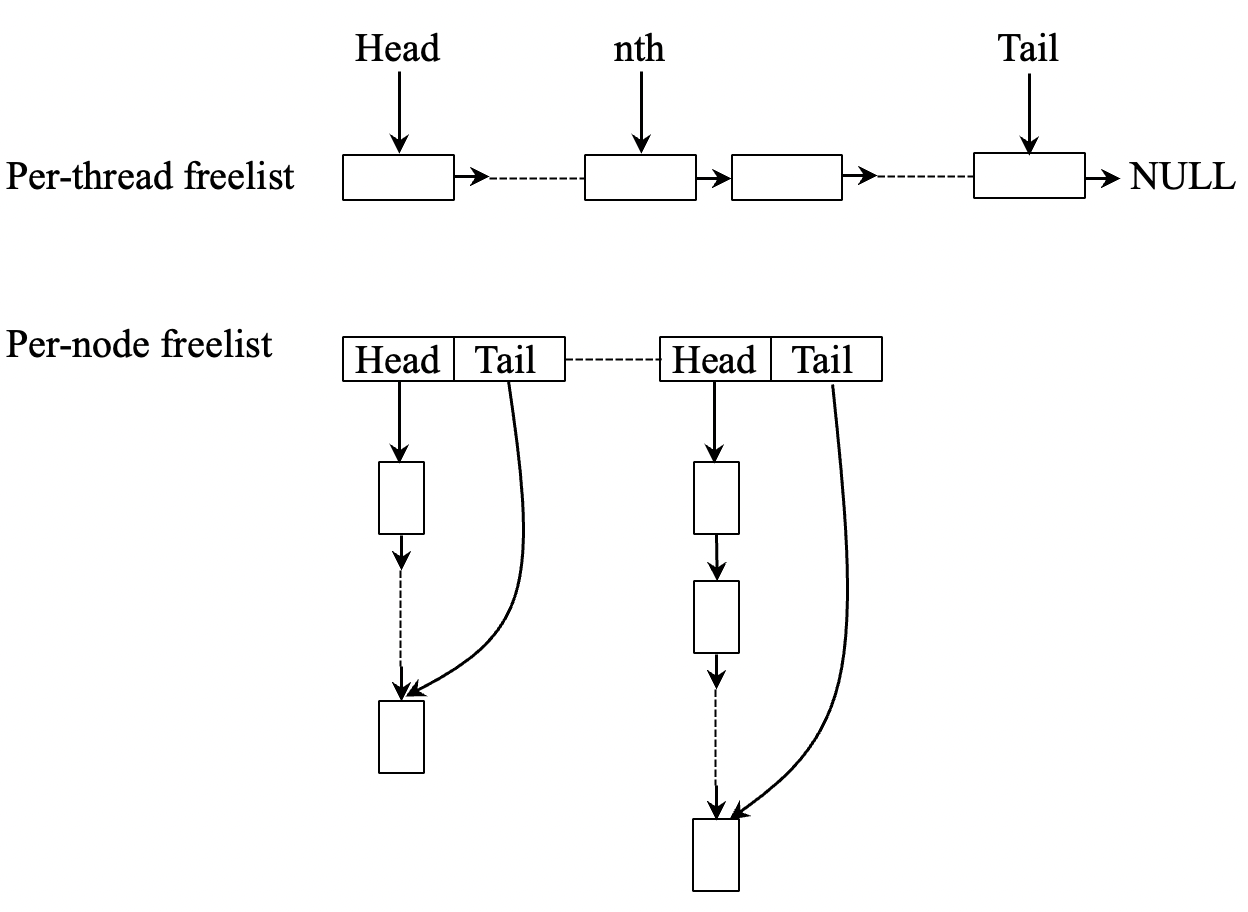
\includegraphics[width=3in]{SC2022/figure/efficient-movement.png}
%\vspace{-0.1in}
\caption{Per-thread freelist and per-node freelist design to achieve efficient object movement.\label{fig:perthreadlist}}
%\vspace{-0.1in}
\end{figure}

\begin{figure*}[!ht]
    \centering
    \includegraphics[width=7in]{SC2022/figure/8-node-parsec-perf.jpg}
    \caption{Performance of different allocators \NEW{on PARSEC and real applications}, where all data\\ is normalized to that of the default Linux allocator. Here, a lower bar indicates a better performance.
    % \todo{To adding the error-bars.}
    \label{fig:perf1}}
 \end{figure*}

\subsubsection{Efficient Object Movement} 
\label{sec:movement}
%It is important to reduce memory blowup that freed objects by one thread cannot be utilized by other threads~\cite{Hoard}. 
\NM{} requires moving freed objects between per-thread and per-node freelists frequently to reduce memory blowup. 
% An efficient mechanism is required to support the frequent movement. 
Existing allocators, such as TCMalloc~\cite{tcmalloc}, traverse the freelist to collect a specified number of objects, and then move all of them at a time, which unfortunately has the following issues: (1) traversing a freed object will bring some unnecessary data to the cache when an allocator is reusing freed objects from the freelist. This loading wastes the cache resources and evicts cache lines with useful content in the future. 
% The loading to the cache is wasted when these objects are moved to other lists later, which will evict cache lines with useful content in the future. 
(2) Existing allocators will typically move recently-freed objects (and hot in cache) to other freelist, which is not good for the performance. (3) The traverse of the shared list may introduce significant lock contention, if multiple threads are waiting to move objects from the shared list. 
\NM{} proposes an efficient mechanism with the following data structures. First, each per-thread freelist maintains two pointers that point to the least recently used objects, shown as the \texttt{Tail} pointer and the $nth$ pointer (counted from the tail) in the upper part of  Fig.~\ref{fig:perthreadlist}. 
This structure avoids the traverse of freelist during the movement, and allows the movement of the least recently used objects (between $(n+1)th$ and $Tail$) to the per-node freelist. After the movement, the \texttt{Tail} pointer will be set to the original $nth$ object. 
Second, \NM{} also proposes a circular array shown in the bottom part of Fig.~\ref{fig:perthreadlist} that helps move objects from the shared per-node  freelist to per-thread freelists. 
%As mentioned above, the per-node freelist could easily become the performance bottleneck, since multiple threads may compete for it concurrently. To address this issue, 
Each per-node freelist actually consists of many sub-lists, where a \texttt{Head} pointer and a \texttt{Tail} pointer point to the header and the tail of each sub-list. When a thread is moving multiple objects from the per-node freelist, it will move all objects in a sub-list (pointed by a pair of \texttt{Head} and \texttt{Tail} pointers) at a time. Therefore, there is no need to traverse the whole list to obtain these objects for the movement, which reduces the contention. 


%Note that this array does not increase the overhead of putting objects. If a thread puts a freed object to this array, the object can be placed into the current sub-list in a constant time. Similarly, a freelist could be appended to the current sub-list in a constant time. 



\begin{comment}
\begin{wrapfigure}{r}{0.6\textwidth}
\centering
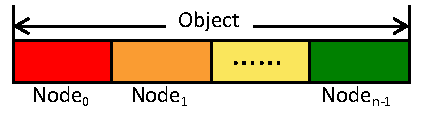
\includegraphics[width=3in]{figure/blockwise}
\vspace{-0.1in}
\caption{Block-wise Memory Allocation\label{fig:blockwise}}
\vspace{-0.1in}
\end{wrapfigure}
\end{comment}

%In theory, private objects of the first thread should not be allocated from the interleaved heap, since that will create remote accesses unnecessarily. Initially, each allocation is treated as a shared one and is allocated from the interleaved heap. Whenever a new thread is created, the allocations are regarded as private ones. Programmers can control whether they want the interleaved support or not based on their applications.


%\NM{} utilizes a simple heuristics to differentiate shared objects from private objects based on allocation callsites: each allocation callsite is treated as a shared one initially, and is allocated from the interleaved heap; Whenever an object is deallocated before creating children threads, indicating such an object is a private one for the main thread, all objects from the corresponding callsite are considered to be private ones, and they are only allocated from the per-node heap afterward. With this heuristics , there is no need to change programs explicitly, although it is more efficient if programmers could provide such information. 

% As mentioned above, \NM{} monitors the  allocation/deallocation pattern of the main thread to identify the share-ability of each callsite. 
%If an allocation callsite is found to be private, then all allocations from this callsite should not allocate from the interleaved heap, but from the normal heap. 
% A challenge is to obtain and compare the callsite of each allocation so that we could determine the heap based on the share-ability. In fact, this may introduce high overhead for applications with large amount of allocations, if using the \texttt{backtrace}~\cite{DBLP:conf/icse/SumnerZWZ10, DBLP:conf/cgo/ZengR0AJ014}. For the performance reason, \NA{} utilizes the sum of the stack position and the return address of the allocation invocation to identify a callsite, called ``\textit{callsite key}''. This combination is able to differentiate callsites correctly if an application does not have allocation wrappers, since the stack position can be utilized to identify the function in the stack and the return address tells the invocation placement inside the same function. If a callsite is misidentified, it will not cause any correctness issue, but with some performance penalties/losses. \NA{} utilizes a hash table to track the status of every callsite. 
 % which is fortunately not very expensive given the limited amount of different callsites. 
 
%Note that the interleaved heap cannot be achieved by using existing NUMA utilities like \texttt{numactl}. Although \texttt{numactl} could also specify memory allocations to be interleaved. However, \texttt{numactl} could only set the policy for a whole application. Instead, \NM{} only utilizes the interleaved heap for shared objects that are allocated in the main thread, not for all objects. 

%\todo{I remove the "Node-Local Metadata" part}

%\subsubsection{Node-Local Metadata} 
%To further reduce remote accesses, \NM{} ensures that all of the metadata is always allocated in the same node. Such metadata includes the metadata for managing per-node lists, per-thread lists, and size class information. Note that ensuring the node-local metadata for per-thread information is only possible when each thread is bound, which is the reason why \NM{} develops the ``binding-based'' approach. Therefore, \NM{} is able to guarantee that all metadata are always allocated in the same node, based on its thread binding as described in Section~\ref{sec:balance}.  
%Such metadata includes per-node and per-thread freelists for different size classes, and freelists for big objects. Similarly, \NM{} utilizes the \texttt{mbind} system call to bind the memory to a specific node.  


%Based on our evaluation, this mechanism reduces most of the memory consumption, with the transparent huge page support by default.  

 %every thread has its own freelists for each size class so that there is no need to acquire the lock when an allocation can be satisfied from its per-thread heap, similar to TCMalloc. That is, two threads will not share the same per-thread heap. However, some applications may create new threads after some threads have exited. \NM{} re-utilizes the memory for these exited threads. Basically, \NM{} intercepts thread joins and cancels so that it can assign heaps of exited threads for newly-created threads, and re-utilize their heaps correspondingly.  


%\paragraph{Transparent Huge Page Support:} During the development, we noticed that excessive memory consumption can be imposed when the OS enables transparent huge pages by default. In order to reduce memory consumption, \NM{} makes multiple threads share the same bag (for the same size class), instead of having a separate bag for each thread. If each thread is running out of the memory, it obtains multiple objects at a time from the corresponding bag. Currently, if a class size is less than one page, then we will at most get objects with the total size of one normal page. Otherwise, it will get 4 objects (with the size less than 64 KB) or 2 objects afterward. Based on our evaluation, this mechanism actually reduces the memory consumption for multiple times for a machine with 128 cores and 8 nodes, with the transparent huge page support by default.  

%\paragraph{Cache Warmup} \NM{} also borrows the cache warmup mechanism of TCMalloc~\cite{tcmalloc}: it will insert all objects in a page into the freelists, if there is no objects in the per-thread freelist. We believe that inserting multiple objects into the freelist will benefit data prefetches, since the insertion is a simple and predictable pattern. With this mechanism, \texttt{raytrace} improves the performance by 10\%. However, this is the only application that we observed such performance improvement. There is no impact on other applications. 

%TCMalloc utilizes a \texttt{mmap} system call to obtain multiple pages (depending on the class size) from the OS each time, when it is running out of the memory for one size class. For such a memory block, TCMalloc inserts all objects of this block into its central freelist at one time. Since TCMalloc utilizes the first word of each object as the pointer for the freelist, this mechanism warms up the cache by referencing the first word of each object during the insertion. According to our observation, this warmup mechanism improves the performance of one application (\texttt{raytrace}) by 10\%. Based on our understanding, the performance improvement is caused by data prefetches, since inserting objects to the freelist has a simple and predictable pattern. \NM{} employs a similar mechanism for small objects with the size less than 256 bytes, and adds all objects inside a page to the per-thread freelist. 

%we propose the combination of per-node heap and per-thread cache. In order to reduce the contention, \NM{} will obtain multiple objects at a time from the per-node heap. 

 
%https://queue.acm.org/detail.cfm?id=2852078
 

\section{Experimental Evaluation}
\label{sec:evaluation}

This section aims to answer the following research questions: 

\begin{itemize}
\item \textbf{Performance:} How is \NM{}'s performance, comparing to existing general allocators and NUMA-aware allocators? (Section~\ref{sec:performance}) 
\item \textbf{Memory Consumption:} What is the memory consumption of \NM{}? (Section~\ref{sec:memory})
\item \textbf{Scalability:} How is the scalability of \NM{}? (Section~\ref{sec:scale})
\item \textbf{Impact of Design Choices:} \NEW{What is the impact of each design choice on} the performance of \NM{}? (Section~\ref{sec:design})	
\end{itemize}



\begin{comment}

\begin{table}[!ht]
 \centering
   \caption{Machine specifications for evaluation
   \label{table:Machine}}
  %\setlength{\tabcolsep}{1.0em}
\begin{tabular}{l | l }
\hline
Category & Information \\ \hline
CPUs/Model 	& Xeon(R) Platinum 8153\\ \hline
CPU Frequency & 2.00GHz\\ \hline
NUMA Nodes  & 8 \\ \hline
Physical Cores  & 8$\times$16 \\ \hline
Node Latency &  \specialcell{local: 1.0 \\ 1 hop: 2.1 \\ 2 hops: 3.1}\\ \hline
Interconnect Bandwidth  & 10.4GT/s\\ \hline
Linux & Debian 10\\ \hline
Compiler &  GCC-8.3.0 \\ \hline
%Memory Bandwidth & 19.87 GB/s & \\ \hline
  \end{tabular}
  %\vspace{-0.4in}
\end{table}
\end{comment}

\textbf{Experimental Setup:}  \NM{} was evaluated on an Intel Xeon(R) Platinum 8153 machine with 8 nodes, where each node has 16 cores.  \NEW{8 nodes are divided into two groups, where the four nodes of each group are fully connected, and there are four links between the two groups. Any two nodes are less than or equal to 2 hops, where the latency of one hop and two hops is 2.1 and 3.1 separately if the latency of local accesses is 1.0}. The machine is installed with 512GB memory. \NEW{Each core has a dedicated L1 (32KB) and L2 (1MB) cache, and cores within a node share a 22MB last-level cache (LLC).} The underlying OS is Linux Debian 10 and the compiler is GCC-8.3.0. In the evaluation, the hyperthreading was turned off, but both transparent huge page and AutoNUMA are enabled. We utilize 128 threads, which is the same as the number of cores of the evaluated machine. \NEW{For OpenMP/MPI applications, we use a hybird MPI + OpenMP mode where the number of MPI processes is equal to the number of nodes and each process has 16 OpenMP threads which is the core number inside a processor.} The performance data shown in this paper is an average of 30 executions, in order to avoid any bias caused by unexpected events.

% \todo{Adding the hardware issue, about node, about LLC} 
% \todo{Adding the glibc's version}

\textbf{Compared Allocators and Evaluated Applications: }  We compare \NM{} with multiple popular allocators, such as the default Linux allocator \NEW{(Glibc-2.28)}~\cite{glibcweb}, TCMalloc~\cite{tcmalloc2},  TCMalloc-NUMA~\cite{tcmallocnuma}, jemalloc-5.2.1~\cite{jemalloc}, Intel TBB-2021.5~\cite{tbb2}, Scalloc-1.0.0~\cite{Scalloc}, and mimalloc\NEW{-1.6.7}~\cite{mimalloc}. Note that we are comparing against TCMalloc's NUMA awareness version (released in July 2021), and the newest version of TBB with NUMA support (released in December 2021). Note that the evaluated TCMalloc already includes TEMERAIRE~\cite{TEMERAIRE}'s huge page support. 
%Among them, TCMalloc, jemalloc, TBB, and mimalloc are commercial allocators designed and maintained by Industrial Giants, like Google, Facebook, Intel, and Microsoft separately. 
We do not include Hoard~\cite{Hoard} as it is not the state-of-art anymore~\cite{Scalloc, mimalloc}. Multithreaded applications chosen to evaluate the performance include PARSEC applications~\cite{parsec}, \NEW{five OpenMP/MPI applications from CORAL-2 Benchmarks~\cite{coral2}, including \texttt{Nekbone}, \texttt{QMCPACK}, \texttt{LAMMPS}, \texttt{AMG} and \texttt{Quicksilver}}, and real applications such as \texttt{Apache httpd-2.4.35}, \texttt{MySQL-5.7.15}, \texttt{Memcached-1.4.25}, \texttt{SQLite-3.12.0}, \texttt{Aget}, \texttt{Pfscan} and \texttt{Pbzip2}.

%Note that we currently have an issue running freqmine, an openmp application, which is excluded right now. 

 \begin{figure}[!h]
    \centering
    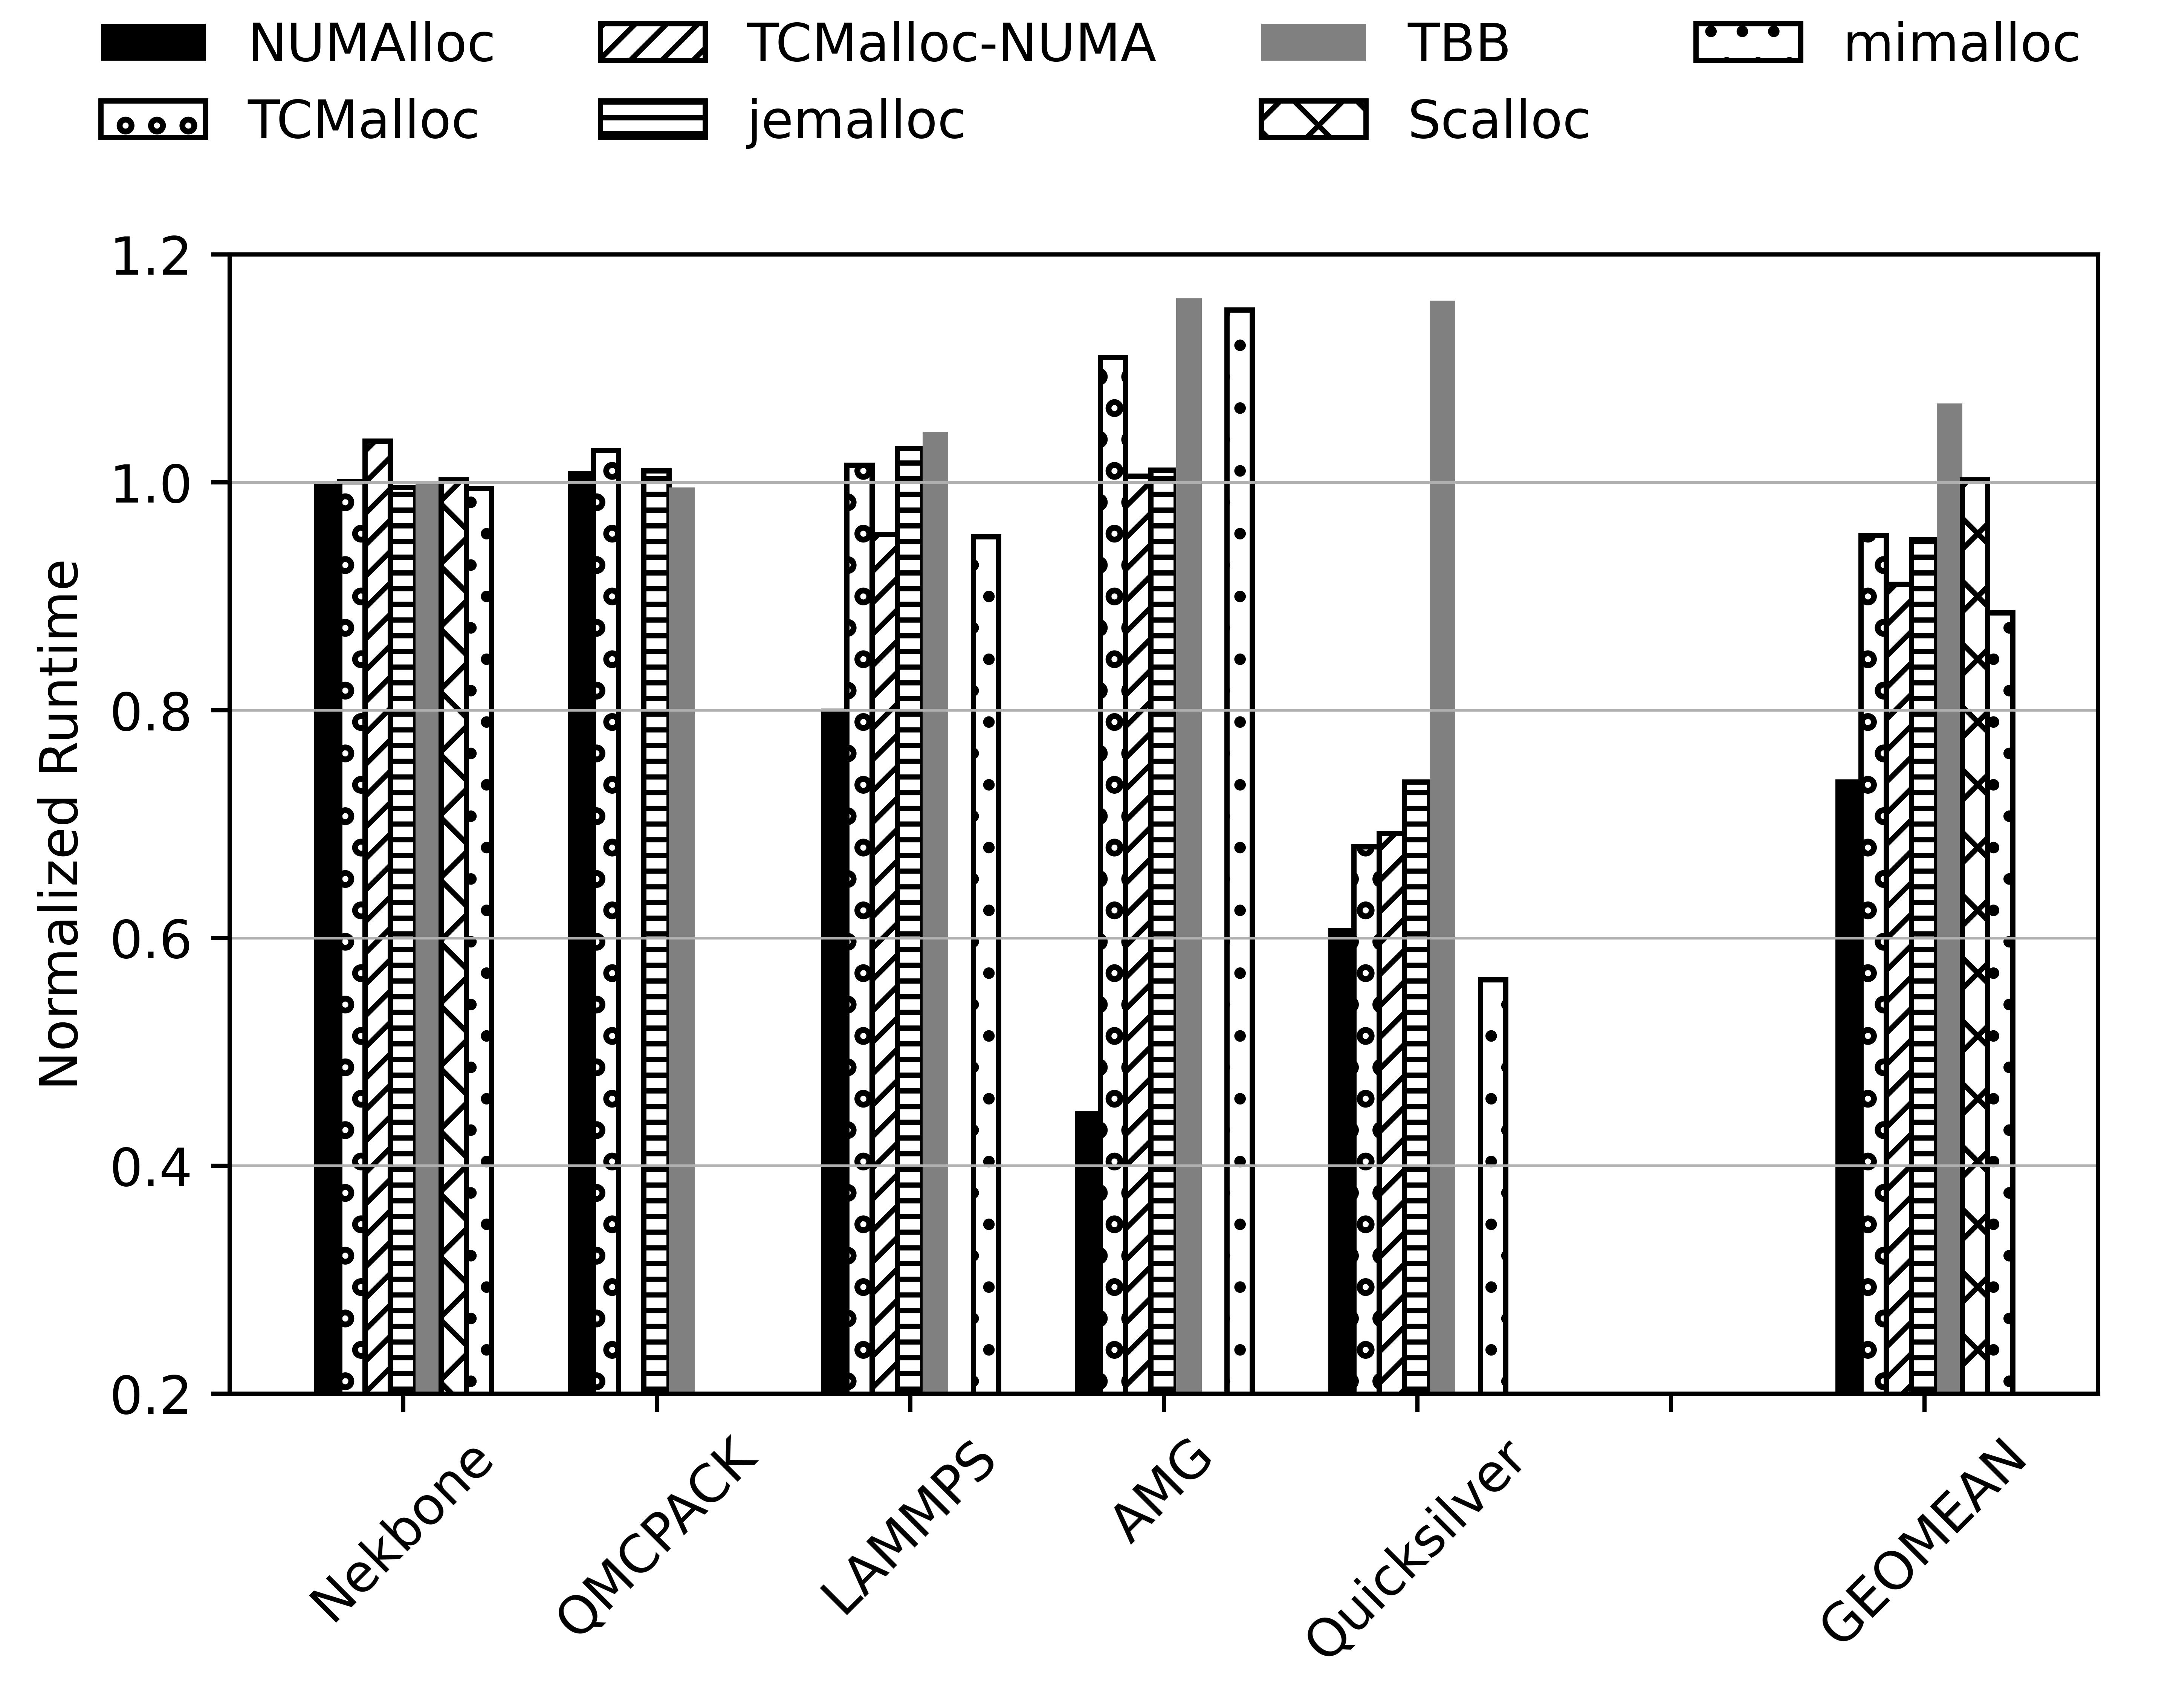
\includegraphics[width=3.5in]{SC2022/figure/8-node-mpi-perf.jpg}
    \caption{\NEW{Performance of different allocators on OpenMP/MPI applications, where all data is normalized to that of the default Linux allocator. Note that some applications are failed to run with some allocators.}
    \label{fig:perf2}}
 \end{figure}

\begin{comment}
\begin{table}[!ht]
 \centering
  %\setlength{\tabcolsep}{1.0em}
\begin{tabular}{c | c | c}
\hline
System & \textbf{Machine A} & \textbf{Machine B} \\ \hline
CPUs/Model & Xeon Gold 6138	& Xeon(R) Platinum 8153\\ \hline
CPU Frequency & 2.10GHz & 2.00GHz\\ \hline
NUMA Nodes & 2 & 8 \\ \hline
Physical Cores & 2$\times$20 & 8$\times$16 \\ \hline
Node Latency & \specialcell{local: 1.0 \\ 1 hop: 2.1} & \specialcell{local: 1.0 \\ 1 hop: 2.1 \\ 2 hops: 3.1}\\ \hline
Interconnect Bandwidth & 8GT/s & 10.4GT/s\\ \hline
Linux & Ubuntu 18.04 & Debian 10\\ \hline
Compiler & GCC-7.5.0 & GCC-8.3.0 \\ \hline
%Memory Bandwidth & 19.87 GB/s & \\ \hline
  \end{tabular}
   \caption{Machine specifications for evaluation
   \label{table:Machine}}
  %\vspace{-0.4in}
\end{table}
\end{comment}

\subsection{Performance Evaluation}
\label{sec:performance}

% PARSEC applications are using native inputs~\cite{parsec}. For \texttt{MySQL}, we use \texttt{sysbench} with 128 threads separately, each issuing 100,000 requests. The \texttt{python-memcached}  is used to exercise \texttt{Memcached}, with 3000 loops to get the sufficient runtime~\cite{memcached}. The \texttt{ab} is used to test \texttt{Apache} server~\cite{apachetest}, by sending 1,000,000 requests in total. \texttt{Aget} is tested by downloading a 30-MB file, and \texttt{Pfscan} is tested by searching  a keyword in a 500MB data. In terms of \texttt{Pbzip2}, we test it by compressing 10 files with 30MB each. Finally, \texttt{SQLite} is tested through a program called \texttt{threadtest3}~\cite{sqlitetest}. 

%\todo{The number of threads of all benchmarks were adjusted according how many cores and nodes in the target machine to make threads could be properly distributed over the nodes and cores, making the number of threads as close as the number of cores. In the test machine, the thread number is 128.}

%In the Hoard~\cite{Hoard} benchmarks, we used 100 iterations and 1,280,000 64-byte objects for threadtest and also we run larson for 10 seconds with 1,000 7-2048 bytes object to cover all size classes in almost all allocators for 10,000 iterations.For false sharing , we used 100,000 inner-loop , 100,000 iterations with 8 bytes objects. 

%The number of threads of all benchmarks were adjusted according how many cores and nodes in the target machine to make threads could be properly distributed over the nodes and cores, making the number of threads as close as the number of cores. Mostly, thread number was 40 in the Machine A and 128 in the Machine B, and I will give the specific number below if it is not this default value. 

The performance results are shown in Fig.~\ref{fig:perf1} and Fig.~\ref{fig:perf2}, where the runtime of each allocator is normalized to that of Linux's default one. \NM{} is configured without the interleaved heap support for most applications, except for \texttt{fluidanimate} and \texttt{streamcluster}. As evaluated in Section~\ref{sec:interleavedheap}, the interleaved heap will significantly improve the performance for these two applications. 
%As further discussed in Section~\ref{sec:interleavedheap}, the interleaved heap may have a harmful performance impact for the serial phases, as it turns some local accesses to remote ones. %Therefore, the data of \texttt{canneal} and \texttt{raytrace} are collected without the interleaved heap. 
%We believe that this option is acceptable, since users could determine easily whether they should disable the interleaved heap: if an application has a large portion in the serial phase, then the interleaved heap should be disabled. 
%The impact of the interleaved heap is further discussed and evaluated in Section~\ref{sec:interleavedheap}. 
 %With the interleaved heap,  allocations from the main thread can be satisfied in remote NUMA nodes, this design may lead to a large number of remote accesses for the serial phase. since both of them spend a large portion of their time (over 62\% and 82\%) in the serial phase (before creating any child thread),
 %These two figures show the best data for these two applications, without the support of the interleaved heap.    
Overall, \NM{} has the best performance among these allocators. In particular, \NM{} is \NEW{15.7\%} faster than the second-best allocator (mimalloc) and \NEW{19.0\%} faster than the default Linux allocator. %\todo{explain why mimalloc is good? why other allocators are not good}
For the best case (e.g., \texttt{fluidanimate}), \NM{} is running up to $5.3\times$ faster than the default Linux allocator, and $6.8\times$ faster than Scalloc.
On average, \NM{} is \NEW{18.2\%}, \NEW{16.3\%}, and \NEW{18.8\%} faster than TCMalloc~\cite{tcmalloc2}, TCMalloc-NUMA~\cite{tcmallocnuma}, Intel TBB~\cite{tbb3}. \NEW{Considering only OpenMP/MPI applications, applications run 26.1\% faster with \NM{} compared with the default Linux allocator, and 16.5\% faster than the second-best allocator (mimalloc).}

\begin{figure}[!h]
    \centering 
    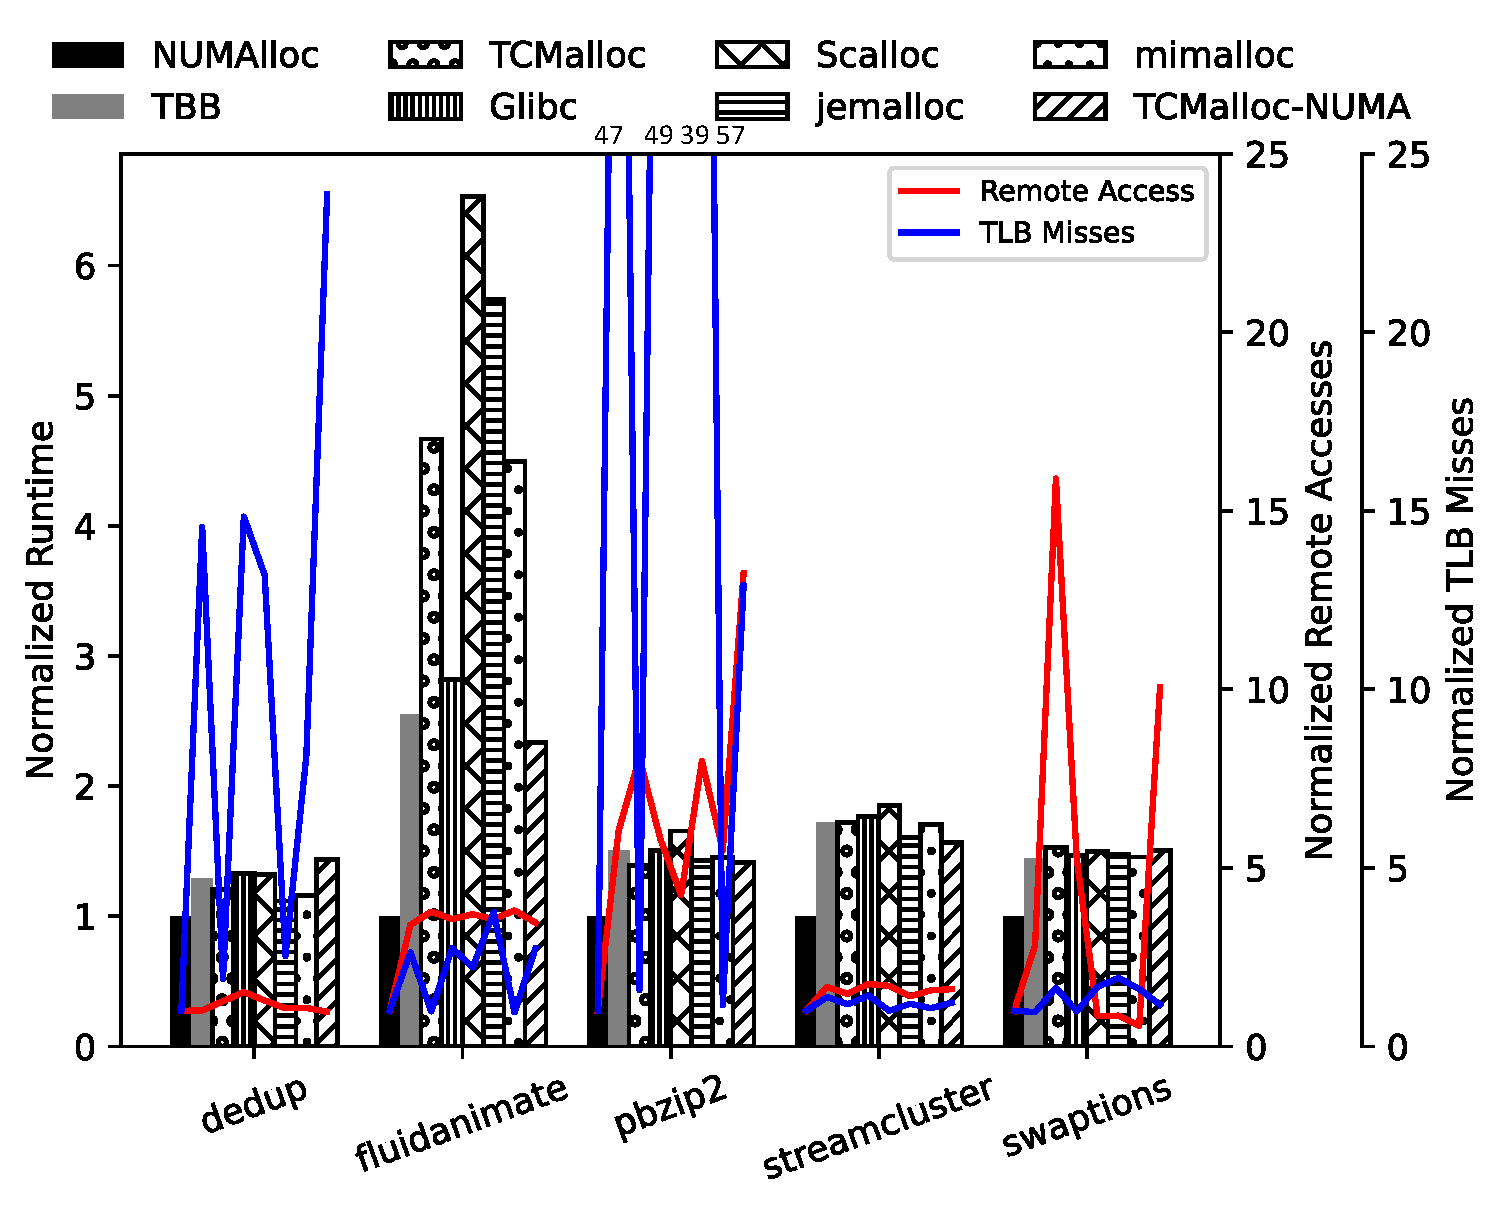
\includegraphics[width=3.5in]{SC2022/figure/remote access.pdf}
    \caption{Normalized runtime, remote accesses, and TLB misses of different allocators (to \NM{}), where the lower is the better. }
    \label{fig:remoteAccess}
\end{figure}

%\NM{} is running \todo{19\%} faster than the default allocator, but does not run significantly slower than other allocators in almost all evaluated applications. For the best case (e.g., \texttt{fluidanimate}), \NM{} is running up to \todo{$6.4\times$} faster than the default Linux allocator.
%The default Linux allocator achieves good performance on the NUMA architecture due to its arena-based design, where each freed object will be returned back to its original arena. This design is integrating well with Linux's first-touch allocation policy~\cite{Lameter:2013:NO:2508834.2513149} to ensure most thread-local allocations. 
% In contrast, other allocators typically utilize a per-thread cache to store objects that are deallocated by the current thread, which may lead to remote accesses as described in Section~\ref{sec:intro}.
% Comparing with the NUMA-aware allocator -- TCMalloc-NUMA~\cite{tcmallocnew}, \NM{} runs \todo{23\%} faster. 
%TCMalloc-NUMA, TCMalloc, TBB, and mimalloc are allocators that are claimed to support the NUMA architecture~\cite{tcmallocnew}. 
%But TCMalloc-NUMA's performance is even worse than that of TCMalloc. Based on our understanding, TCMalloc-NUMA is based on TCMalloc-0.97 (released in 2008), which does not have new features of TCMalloc-2.7 (the version for our evaluation). 
% mimalloc only has the very basic NUMA support, which is the reason why it is not performing as well as \NM{}. TCMalloc and TBB are allocators that are claimed to support the NUMA architecture~\cite{tcmalloc2, tbb3}, but \NM{} is \todo{21\%} faster than both of them.

As shown in Fig.~\ref{fig:perf1}, \NM{} has a significant performance improvement (over 25\%) in the following applications, including \texttt{dedup}, \texttt{fluidanimate}, \texttt{pbzip2}, \texttt{streamcluster}, and \texttt{swaptions}. For these applications, we further examine the number of remote accesses and TLB misses to confirm whether \NM{} significantly reduces them. 
% By ensuring the full locality of memory accesses, \NM{} is expected to reduce the number of remote accesses. \NM{} will reduce the TLB misses, since it takes the advantage of transparent huge pages.  
We utilize the \texttt{perf}\NEW{~\cite{perfweb} (version 4.19), a Linux performance profiling tool,} to collect these numbers. 
% Figure~\ref{fig:perf} shows that \NM{} has a similar or better performance than the default allocator in almost all applications. Further, it has a significant performance improvement (over 20\%) in the following applications, including \texttt{canneal}, \texttt{dedup}, \texttt{fluidanimate}, \texttt{streamcluster}, and \texttt{pbzip2}. Among them, \NM{} has a better performance for \texttt{fluidanimate}, due to the following reasons. First, the interleaved heap contributes to $3.23\times$ performance speedup, as shown in Figure~\ref{fig:interleavedheap}. Second, node-balanced thread binding improves the performance by over $4\times$. 
% \textbf{Confirming the number of remote accesses:} We further examine the number of remote accesses to confirm whether \NM{} significantly reduces them due to its design. We utilize the \texttt{perf} to collect the number of remote accesses (both load and store) on these applications when they are running with all allocators. 
%In our machine, we can collect these numbers using the following command: \texttt{perf stat -e node-load-misses,node-store-misses,dTLB-store-misses,dTLB-load-misses} 
The results are shown in Fig.~\ref{fig:remoteAccess}, which includes the performance (shown as bars), remote accesses (red lines), and TLB misses (blue lines) together for a better comparison. 
% For all these data, the lower is better. 
Overall, \NM{} has either a lower number of remote accesses or TLB misses than other allocators, which explains why \NM{} is the fastest on these applications. We also notice that both \NM{} and TCMalloc have a lower number of TLB misses, as they have the support for huge pages.   

%We only use five applications that \NM{} has significantly better performance than other allocators.
\NM{} significantly reduces the number of remote accesses for three applications, \texttt{fluidanimate}, \texttt{pbzip2}, and \texttt{streamcluster}. Let us utilize \texttt{fluidanimate} as an example, where \NM{} is running $2.9\times$ faster than the default Linux allocator and $4.6\times$ faster than TCMalloc. Fig.~\ref{fig:remoteAccess} shows that the number of remote accesses for the default allocator and TCMalloc is $3.6\times$ and $3.8\times$ more than \NM{}. However, there is no much difference in the number of remote accesses for \texttt{dedup} and \texttt{swaptions} compared with some allocators. Based on our investigation, \NM{} is running faster than others due to the reduction of TLB misses instead. 
\NEW{We also conduct such experiments on the OpenMP/MPI applications shown in Fig.~\ref{fig:perf2}. Compared with the second-best allocator (mimalloc), the remote accesses of \NM{} are reduced by $13.9\times$ and the TLB misses are reduced by $1.08\times$ on average. The data for other allocators are similar or even worse. This further confirms that \NM{} can reduce the number of remote accesses as well as TLB misses, thus improving the performance.}

\NM{}'s big reduction of remote accesses can be attributed to the following factors: its thread binding avoids unnecessary remote accesses; its metadata is placed on the local node, based on the binding design; its origin-aware memory allocation ensures locality of memory allocations.
For TLB misses, \NM{} is orders of magnitude lower than other allocators (except TCMalloc) for \texttt{pbzip2}. Especially, the default allocator and jemalloc have $48\times$ or $57\times$ more TLB misses. Interestingly, the performance difference of \texttt{pbzip2} is even smaller than \texttt{fluidanimate}, given the large difference in TLB misses. Based on our understanding, \texttt{pbzip2} is an IO-bound application so that the computation difference does not have a large impact on its overall performance. 
%\NM{} has a  more close to those of other allocators for \texttt{swaptions}.
Overall, \NM{} either has fewer remote accesses or fewer TLB misses, which \NEW{are the reasons that \NM{} has} better performance than other allocators on these applications. 

%\renewcommand{\arraystretch}{1.5}
\begin{table}[tp]
\footnotesize
	\setlength{\tabcolsep}{0.3em}
  \centering
    \begin{tabular}{|l|r|r|r|r|r|r|r|}
    \hline
    \multirow{2}{*}{Apps}&
    \multicolumn{7}{c|}{Memory Usage (MB)}\\
    \cline{2-8}
    &Linux&\NM{}&TcM&TcM-N&jem&TBB&Scalloc \\ \hline
    \hline
    blackscholes&615&509&621&623&633&615&630\\ \hline
    bodytrack&37&161&45&46&570&37&1994\\ \hline
    canneal&888&879&774&757&1294&888&36149\\ \hline
    dedup&912&1236&983&1023&1389&912&8556\\ \hline
    facesim&560&500&603&601&1133&547&3056\\ \hline
    ferret&184&493&195&183&596&184&3377\\ \hline
    fluidanimate&470&392&483&484&481&470&3437\\ \hline
    raytrace&1288&1472&1092&1543&1287&1288&4398\\ \hline
    streamcluster&113&105&123&121&127&113&193\\ \hline
    swaptions&33&268&16&21&540&37&1817\\ \hline
    vips&228&536&248&269&778&227&3681\\ \hline
    x264&2859&2721&3047&3064&3719&2859&5402\\ \hline \hline  
    Aget&8&74&11&10&93&8&80 \\ \hline
    Apache&8&34&10&9&10&4&42\\ \hline
    Memcached&16&80&25&24&41&18&263\\ \hline
    Mysql&277&732&314&315&500&276& N/A \\ \hline
    Pbzip2&463&747&817&813&1121&454&4881 \\ \hline
    Pfscan&522&542&528&528&535&522&554\\ \hline
    Sqlite3&45&284&60&75&139&44&681 \\ \hline
    \hline
    Total&{\bf 9527}&{\bf 11763}&{\bf 9993}&{\bf 10510}&{\bf 14986}&{\bf 9502}&{\bf 79190}\cr\hline
    \end{tabular}
  \caption{Memory consumption of different allocators. Here, TcM stands for TcMalloc, TcM-N is TcMalloc-NUMA, and jem is jemalloc. \label{tab:memory_consumption}}
\end{table}


To further validate the effectiveness of \NM{}, we also evaluate it on the Rodinia OpenMP benchmark suite~\cite{che2009rodinia}. According to the results, applications using \NM{} gain an average speedup of $2.33\times$ compared to the second-best allocator (mimalloc), and $2.44\times$ speedup compared to the default Linux allocator, which indicates that \NM{} also performs well on OpenMP applications. Due to the page limit, we do not show the runtime of each application in this paper. 

%However, there is no much difference in the number of remote accesses for \texttt{dedup} and \texttt{swaptions} compared with some allocators.  When transparent huge page support is enabled, \NM{} utilizes huge pages instead of small pages, leading to fewer TLB misses. For example, for \texttt{dedup}, \NM{}'s TLB misses is $2.82\times$ lower than that of TCMalloc-NUMA, under the similar number of remote accesses.

% \todo{check if there is a true causality between the amount of reduced remote access and the amount of performance improvement; Better insight into some of the experiments to understand why in about 40\% of the cases NUMAlloc doesn't clearly beat other allocators.}




%For TLB misses, typically both both \NM{} and TCMalloc have lower TLB misses than others, as they all take advantage of huge pages. For \texttt{pbzip2}, other allocators (e.g., TBB, glibc, Scalloc, and jemalloc) could be dozens of larger than \NM{}'s. \todo{We can also observe this trend in \texttt{dedup} application.}

% \NM{} also has much less TLB misses on \texttt{dedup} application.

%data in https://docs.google.com/spreadsheets/d/1WqWH5J7CcQuV8Vs4HnqRSC7TZpgQGPB9Gh2knHPSZPU/edit?usp=sharing
%We also observe some similar results for other applications. For \texttt{dedup}, the \texttt{glibc} allocator introduces 17850 time more TLB misses than \NM{}. Note that we only collect these two factors here, where the performance of allocators can be caused by other reasons, such as memory management operations.

%Further, \NM{} allocates a large chunk of memory initially, then the OS tends to utilize huge pages if possible, although this mechanism may introduce more memory consumption as evaluated in Section~\ref{sec:memory}.  


%\todo{Change "Performance" to runtime, also change the the performance/remote accesses" scale to 8, maybe put NUMAlloc to the first, change TcMalloc to TCMalloc. }

\begin{comment}
\begin{table}[htp]
    \centering
    \footnotesize
    \begin{tabular}{l|c| c|c|c|c|c|c|c|c}
    \multicolumn{2}{c|}{Application} & glibc & \NM{} & TCM & TCM-NUMA & jemalloc & TBB & Scalloc & mimalloc \\ \hline
    \multirow{2}{*}{canneal} & Remote & 772 & 613 & 718   & 626 & 690 & 752 & 655 & 709\\ \cline{2-10}
    & TLB Misses &  & 975  &    &  &1876  & 1910 & 1836 & 1876 \\ \hline
    \multirow{2}{*}{dedup}  & Remote & 35.7 & 23.8 & 23.2 & 32.6 & & 29.9 & 28.4 & 23.7\\ \cline{2-10}
     & TLB &  & 21.6 &    &  & & 31.1 & 42.0  & 19.2\\ \hline
    \multirow{2}{*}{fluidanimate} & Remote  & 784 & 145 & 755 & 902 & & 741 & 798 & 749\\ \cline{2-10}
    5.2
   & TLB  &  & 11.9  &    &  & & 116 & 137 & 100\\ \hline
    \multirow{2}{*}{streamcluster} & Remote  & 762 & 571 & 602 & 548 & & 768 & 497 & 570\\ \cline{2-10}
    &  TLB  &  & 12.1 &    &  & & 1455 & 1410 &  1432\\ \hline
    \multirow{2}{*}{pbzip2} & Remote  &  59.3 & 15.2 & 102 & 98.8 & & 62.5 & 45.8 & 60.4\\ \cline{2-10}
    & TLB &  & 0.8 &    &  & & 98.1 & 66.8 & 26.7 \\ \hline
    \end{tabular}
    \caption{TLB misses when using different allocators. The data shown is mega. }
    \label{tab:characteristics}
\end{table}

\end{comment}

%Table~\ref{tab:characteristics} shows that \NM{} significantly reduces the number of remote accesses and TLB misses due to its region-based design. 

%\todo{Hanmei: maybe we need to get the data on these applications. perf stat -e node-loads, node-load-misses, node-stores, node-store-misses ./APP a.out}



%We  can see that the average value of \NM{} is 0.97 in Machine A and 0.92 in Machine B and it is always the best among all other allocators. The reason that \NM{} got better performance in Machine B is that there are more nodes and more cores in Machine B, which means \NM{} could be very helpful to better to take use hardware resource of multi nodes and cores. but we could get amazing improvement if we shutdown interleaved heap in \NM{} and we will give the data in following sections.In the figure ~\ref{8node-parsec-perf}, we could see more exciting improvement from \NM{}, with average normalized value of 0.92 that is not only the best but also far aware better than all the rest allocators that TCMalloc and jemalloc got 0.99, TCMalloc-NUMA and TBB got roughly 1.07 and 1.01 separately. And also, we can see that the performance of \NM{} is the best for almost each single applications, especially it got 0.17 in fluidanimate and 0.66 in streamcluster which is far better than any of other allocators. As the same thing, the performance of ratrace and canneal is not good here, we will talk about it later after we shut down the interleaved heap.


%In the figure ~\ref{hoard-perf}, we show the normalized performance for Hoard benchmarks in Machine A and Machine B separately. We can see from figure ~\ref{hoard-perf} that the average value of \NM{} is also the best, which is 0.47 that means 2 times faster than default Linux Allocator, and jemalloc got 0.7 and Scalloc got 0.9. In the threadtest, the normalized value of \NM{} is 0.19 , far better than any of others, which means there are few central free list competitions, mainly contributed by properly node management and low overheads operations. For false sharing, \NM{}'s performance is also almost the best as same as Scalloc and jemalloc, which means they could handle false sharing issues very properly. In the larson, \NM{} and TCMalloc are the best, which mainly contributed by their low overheads for allocation and remote de-allocation, but due to our better node management, \NM{} could be better in the Machine B which will be mentioned later. In the figure ~\ref{hoard-perf}, we can also see that \NM{} got lowest average normalized value:0.33, significantly smaller than any of others that TBB got 0.99, Scalloc and jemalloc got roughly 1.14. And also, \NM{} and Scalloc could handle false sharing issue very well, and \NM{} could extremely well reduce central free list competition in threadtest. In larson, \NM{} is the best due to its properly multi-node management. 

\subsection{Memory Consumption}
\label{sec:memory}

We also measure the memory consumption of these allocators, as shown in Table~\ref{tab:memory_consumption}.
%For non-server applications, such as \texttt{Aget}, \texttt{Pbscanf}, \texttt{Pbzip2} and all PARSEC applications, we utilized the sum of the \texttt{maxresident} output from the \texttt{time} utility and the size of huge pages, since the \texttt{time }output does not include huge pages. 
%To determine the size of huge pages, a script is used to periodically collect the number of huge pages by reading from \texttt{/proc/meminfo} file, and then the maximum value of huge pages is used. \todo{removed. This is for mmap's huge page, THP usage is counted}
%For server applications, such as \texttt{MySQL}, \texttt{SQLite}, and \texttt{Memcached}, \texttt{Apache}, the maximum memory is collected by the sum of both \texttt{VmHWM} and \texttt{HugetlbPages} fields from \texttt{/proc/PID/status} file, after the corresponding client exits. 
%We always reboot server applications for each single test. 
% Memory overhead is listed in Table~\ref{tab:memory_consumption}.
Overall, the Glibc allocator has the smallest memory consumption, and TBB is the second-best one. \NM{}'s total memory consumption is around 12\% more than that of the default Linux allocator, but it is similar to TCMalloc and is better than jemalloc and mimalloc. It is far better than scalloc when THP is enabled. When only considering applications with a large footprint, over 500MB, \NM{} introduces 10\% memory overhead on average, which is also comparable to TCMalloc.  
%Scalloc is the worst one in terms of memory consumption, which consumes around  $8.3\times$ more memory that that of TBB.  

\NM{}'s \NEW{higher} memory consumption is mainly caused by its use of huge pages. When enabling transparent huge pages, an application will use 2MB of physical memory even if it only allocates a small object (e.g., 8 bytes). As shown in the column of ``w/o THP'' of Table~\ref{tab:memory_consumption}, when the transparent huge page support is disabled, \NM{}'s memory overhead is actually comparable to Glibc and Intel TBB, where the total memory consumption is decreased from 15210 MB to 13364 MB. That is, \NM{} imposes a similar memory overhead when not using huge pages. We expect that \NM{}'s memory consumption can be further reduced by utilizing some complicated mechanisms proposed by TEMERAIRE~\cite{TEMERAIRE} (TCMalloc).   

The memory consumption of \NM{} is almost $7\times$ lower than Scalloc with huge page support. Similarly, Scalloc allocates a big region of virtual memory from the underlying OS initially, which will be backed by huge pages physically. \NM{}'s memory consumption is much lower due to its ``incremental sharing'' mechanism. Comparing to Scalloc, \NM{} makes all threads (with different size classes) in the same node share the same huge page, as described in Section~\ref{sec:hugepages}, which effectively reduces its memory consumption. 
%In total, Scalloc utilizes $7\times$ more memory when transparent huge page support is enabled.  

%We further confirmed the memory consumption when transparent huge page support is disabled, which can be seen in Table~\ref{tab:memory_consumption}. In this case, \NM{}'s total memory overhead is comparable to the default Linux allocator. Other allocators will not be affected much by transparent huge pages, since they typically obtain a small chunk from the OS each time, less than the size of a huge page (2MB), then the OS will not allocate physical pages from huge pages by default. Therefore, we believe that \NM{}'s memory consumption is acceptable. 

%Second, \NM{} may not return the memory to the OS immediately for large pages. However, we believe that its memory consumption is acceptable. 
  %which actually shows the worst case for \NM{}. The OS will utilize huge pages if a memory area is larger than the size of a huge page (2MB). Since \NM{} utilizes \texttt{mmap} to allocate a huge chunk of virtual memory, this makes all heap memory for real objects will be allocated from huge pages. Currently, \NM{} also utilizes 1MB as the superblock for each size class, making objects of a size class that will occupy at least 1MB even if it only uses an object inside. 
 % Therefore, an application with many size classes will waste more memory. \NM{} makes all threads share the same bag for each size class, as described in Section~\ref{sec: others}, which effectively reduces its memory consumption by multiple times. 
 
 %Scalloc has excessive memory consumption, since its design does not support transparent huge pages very well. Similar to \NM{}, Scalloc utilizes a \texttt{mmap} system call to allocate a continuous huge region of virtual memory from the underlying OS. Since every thread will get a virtual span (2MB) for each size class in Scalloc, it will utilize 2MB physical memory even if only a word is touched. Differently, \NM{} avoids this issue as described in Section~\ref{sec: others}.
% the OS will assign a huge page when transparent huge page is enabled by default. Thus, if only one object is allocated from a size class, 
 
\begin{comment}


In Figure~\ref{2node-hoard-mem}, the average normalized value of \NM{} is larger than others, but actually not too much, which is 2.3 for \NM{}, 1.9 for TCMalloc-NUMA and 1.8 for TCMalloc. It is because that proper node management is utilized in \NM{} and also in TCMalloc-NUMA, so that each node also preserves some memory not only thread locals. But we believe that these little more memory overheads are totally acceptable. It is also the same thing for Figure 10, that the average value for \NM{} is a little higher than others, which is 5.3. But in this 8 nodes machine, \NM{} is not the worst, that Scalloc's average value is 25 and jemalloc is 9.4. One main reason that the value of \NM{} is smaller is that we use mini-size bags in \NM{} which is less than the size of one page for small objects and also memories for small objects are shared per node but per cores in Scalloc.
	
\end{comment}

\begin{figure*}[!th]
    \centering
    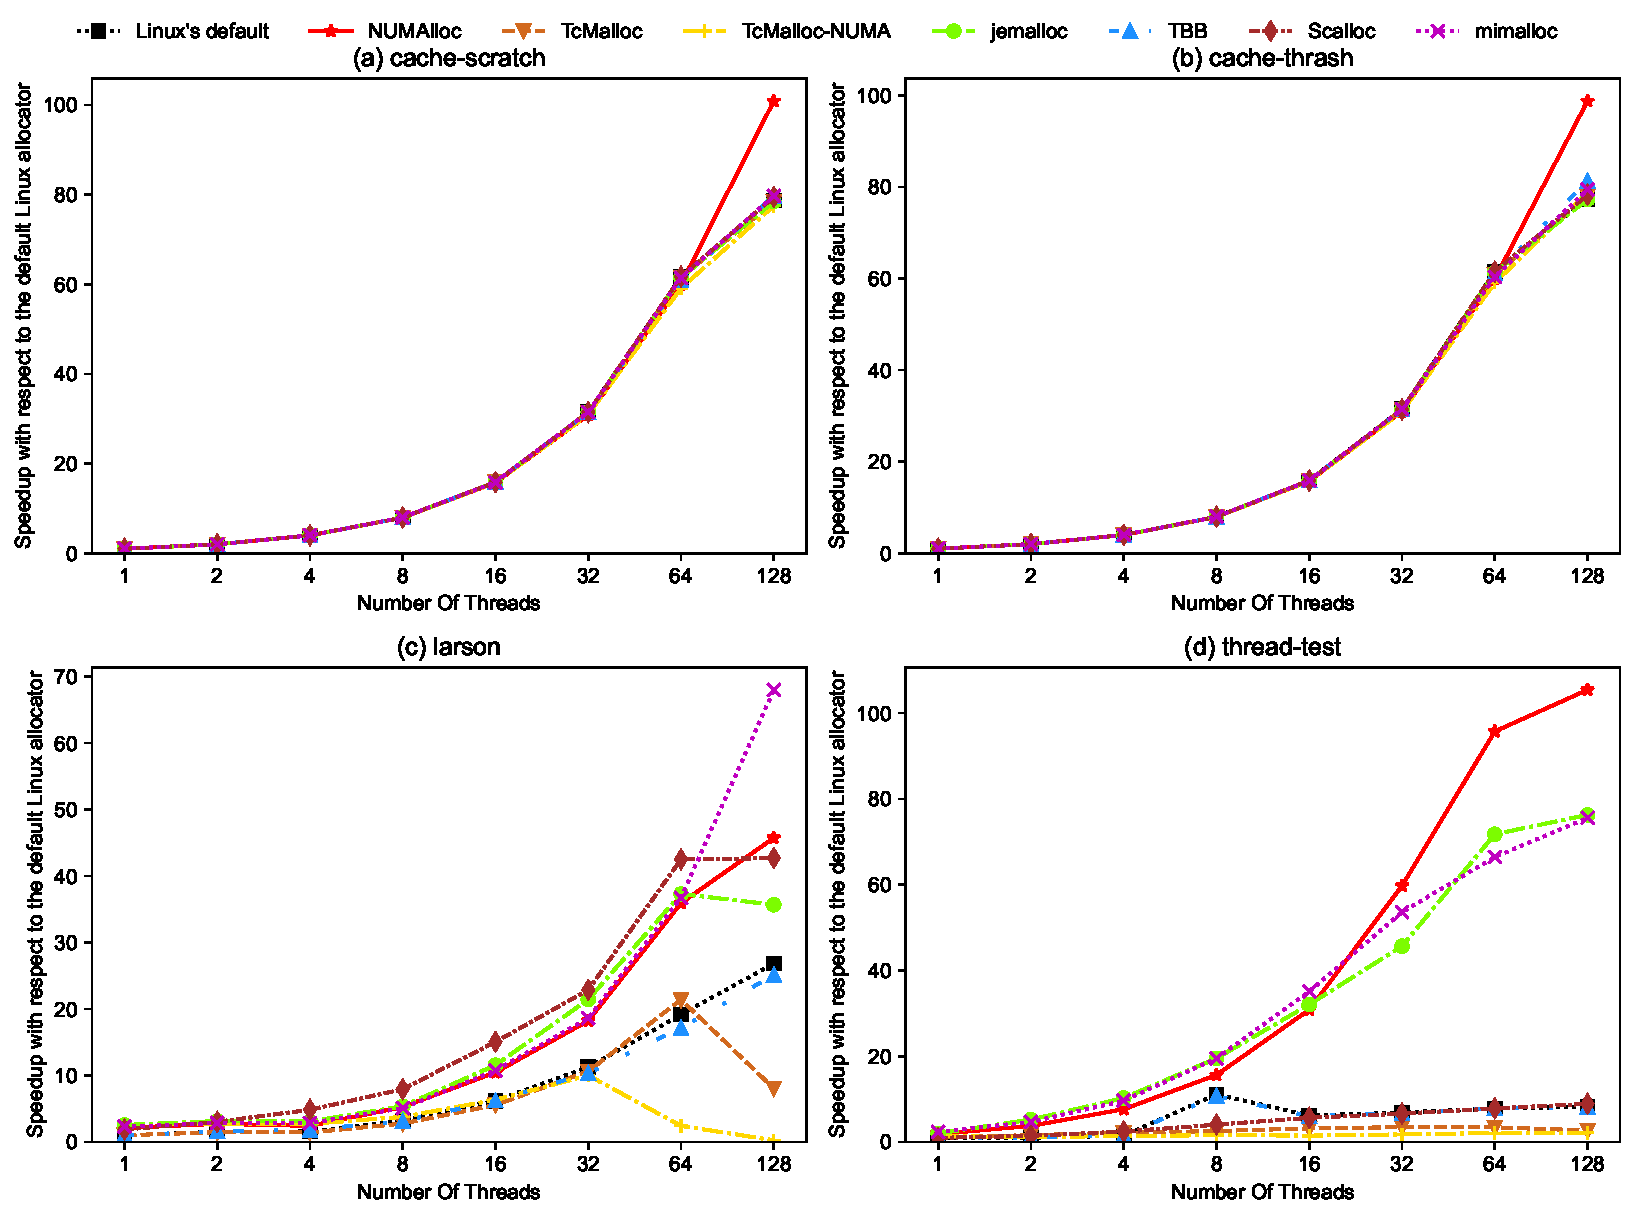
\includegraphics[width=6.1in]{figure/sythentic-scalobility-new.pdf}
    \caption{Scalability evaluation of different allocators.\\ All data is normalized to the runtime of the default Linux allocator with one thread.}
    \label{sythentic-scalability}
\end{figure*}

\begin{figure}[!h]
\centering
\subfloat[Normalized runtime without thread binding for Glibc and TCMalloc, where the lower is the better.]{
  \includegraphics[width=3.2in]{SC2022/figure/threadbinding1.jpg}
}

\subfloat[Normalized runtime with node-interleaved and node-saturate binding for \NM{}, where the lower is the better.]{
  \includegraphics[width=3.2in]{SC2022/figure/threadbinding2.jpg}
}
\caption{Performance impact of thread binding.}
\label{binding-pthread-scalibity}
\end{figure}

\begin{figure}[!ht]
    \centering
    \includegraphics[width=3.2in]{SC2022/figure/hugepage.jpg}
    \caption{Normalized runtime with and without THP for \NM{}.  \label{fig:hugepage}}
\end{figure}

\begin{figure}[!ht]
    \centering
    \includegraphics[width=3.2in]{SC2022/figure/interleavedheap.jpg}
    \caption{Normalized runtime with and without the interleaved heap for \NM{}.  \label{fig:interleavedheap}}
\end{figure}


\subsection{Scalability}
\label{sec:scale}

%We also evaluated the scalability of different allocators. 

To validate the scalability of \NM{}, we use four synthetic applications from Hoard~\cite{Hoard}, including \texttt{threadtest}, \texttt{larson}~\cite{Larson}, \texttt{cache-scratch} and \texttt{cache-slash}, which is also employed by existing work~\cite{Scalloc}. We do not use the same applications in Section~\ref{sec:evaluation}, as they are not scalable by design.
%We have verified blacksholes, bodytrack, canneal, and raytrace.
For instance, raytrace has no performance difference when running with 16 threads or 40 threads.
%Therefore, we are using four synthetic applications from Hoard~\cite{Hoard}, including \texttt{threadtest}, \texttt{larson}~\cite{Larson}, \texttt{cache-scratch} and \texttt{cache-slash}, which is also employed by existing work~\cite{Scalloc}. \texttt{larson} simulates a multithreaded server that could respond to requests from different clients, and \texttt{threadtest} is an application that performs a large number of allocations and deallocations within a specified number of threads. Both \texttt{cache-scratch} and \texttt{cache-thrash} test false sharing issues that can be introduced by allocators, where multiple threads are getting and accessing different objects in the same cache line.  
%Passive false sharing is introduced upon deallocations, where a freed object can be utilized by another thread. In contrast, active false sharing is introduced during the initial allocations, where multiple continuous objects sharing the same cache line are allocated to different threads. The synthetic applications have a better scalability by design than other evaluated applications in the last section. 
%Since other allocators cannot specify the configuration, we only evaluate the scalability with different number of threads. 
In the evaluation, we maximize the number of threads on each node for \NM{}. For instance, 32 threads will use 2 nodes, as each node has 16 cores. For other allocators, we only specify the number of threads, and it is up to the OS to determine the scheduling. 
%The corresponding data is shown in Fig.\ref{sythentic-scalability}. All data are normalized to the data of one thread of the Linux's default allocator, where the higher is better.
 
Fig.\ref{sythentic-scalability} illustrates different allocators' performance speedup with the increasing number of threads. All data is normalized to the runtime of Linux's default allocator under one thread. Overall, \NM{} has the best performance when the number of threads is 128. Its average speedup is $88\times$, compared to Linux's allocator with one thread, while the second-best allocator -- \texttt{mimalloc} -- has $75\times$ speedup. In contrast, the default Linux allocator only has the speedup of $49\times$. That is, \NM{} has the best scalability compared to other allocators.
%When computing the speedup using the data of one thread of each allocator, \NM{}'s average speedup is $65\times$, while the second-best one is $54\times$. 

\NEW{Among these applications, both \texttt{cache-scratch} and \texttt{cache-thrash} test false sharing issues that can be introduced by allocators, where multiple threads access different objects in the same cache line. For both applications, \NM{} has similar scalability compared to other allocators up to 64 threads. But when it comes to 128 threads, \NM{} outperforms all other allocators. According to our investigation, other allocators suffer from false sharing issues while \NM{} avoids the problem and thus has better performance.}
% has a much lower cache miss rate compared to other allocators.}
In these four applications, \NM{} only performs worse than mimalloc for \texttt{larson} with 128 threads. \NEW{\texttt{larson} simulates a multithreaded server that can respond to requests from different clients. In this application, each thread is given a set of objects, and they perform random deallocations and allocations on these objects within a round, and finally pass the objects to the next thread before terminating. Unlike other applications, \texttt{larson} runs for a fixed time and we use a throughput metric (the number of memory allocations per second) to measure the performance. Remote deallocations are quite common for this application, as local objects can be passed to other remote threads. Therefore, the performance of \texttt{larson} is sensitive to the memory recycling mechanisms of the allocator, as observed in the existing work~\cite{Scalloc, scalableallocator}. As discussed in Section~\ref{sec:origin}, remote object's deallocation is managed by the original node's freelist to ensure the locality. This freelist is shared among all threads running on this node, which can become a bottleneck when serving multiple deallocations at the same time. Nevertheless, \NM{} still performs better than most allocators on \texttt{larson} and can scale to 128 threads.}
% Although most deallocations are performed by the allocating thread which occurs on the local node, remote deallocations are also common, as local objects can be passed to other remote threads. Therefore, } 
% we do not know the exact reason for this, but \NM{} is still good enough against other allocators. \NEW{reason!}
% but it performs better against mimalloc for other applications. 
All of these data indicate that \NM{} is scalable to 128 cores. 
%We don't know the exact reason for this.

% \todo{the scalability disadvantage of NUMAlloc at 32 or 64 threads, or > 128 threads}

% \todo{Previous we have analysis of TCMalloc on two cache applications, but I think it's not representative as larson and thread-test}

%Among these applications, \texttt{cache-scratch} tests passive false sharing, and \texttt{cache-thrash} tests active false sharing. False sharing occurs when multiple threads are concurrently accessing different words in the same cache line. 
%Passive false sharing is introduced upon deallocations, where a freed object can be utilized by another thread. In contrast, active false sharing is introduced during the initial allocations, where multiple continuous objects sharing the same cache line are allocated to different threads. 
%For these false sharing tests, we use 100,000 inner-loop, and 100,000 iterations with 8-byte objects.

\begin{comment}
Among these applications, \texttt{cache-scratch} tests passive false sharing, and \texttt{cache-thrash} tests active false sharing. TCMalloc has serious issues of both active and passive false sharing issues, which is the major reason that it does not perform well on both applications. 
\NM{} will not introduce active false sharing, since each thread will get a page of objects initially. Although \NM{} might introduce passive false sharing due to its per-thread cache design, it avoids remote allocations across the node. 
%We believe that is the major reason for its better performance. Other allocators do not have such mechanisms. That is the reason why 
\NM{} is one of the best allocators for \texttt{cache-scratch}, and achieves much better speedup than all other allocators in \texttt{cache-thrash} (30\% faster than the second-best one), as shown in Figure~\ref{sythentic-scalability}. 
\end{comment} 
 %\texttt{larson} is to simulate a multithreaded server that could respond to requests from different clients. \NM{} is around 16\% faster than the second-best allocator--TCMalloc.   \texttt{threadtest} is an application that performs a large number of allocations and deallocations within a specified number of threads. \NM{} is $2.6\times$ faster than the second-best one (jemalloc), when there are 128 threads.
 %Each thread will receive a random number of objects in the beginning, perform a random number of allocation and deallocations to simulate the handler for processing requests, and then pass objects to the next thread. We test \texttt{larson} for 10 seconds with 1,000 objects for 10,000 iterations, where each allocation is between 7 bytes and 2048 bytes. 
 %As shown in Fig.~\ref{sythentic-scalability},  



%Also, it allows to specify how much work to be done between each allocation and deallocation. For \texttt{threadtest}, we use 100 iterations, 1,280,000 allocations, 0 work, and 64-byte objects (for the allocation).  This benchmark will stressfully test the performance overhead of allocation and deallocation. For this application, 
 %since every thread will has its own heap and it only imposes some when getting objects from the shared bag. But \NM{} obtains a number of objects at a time, at the page level, which significant reduce the possibility of contention. 


%On average,  \NM{} is running 79\% faster than the second-best one (Scalloc), and $2.2\times$ faster than the default Linux allocator. Multiple reasons contribute to the good performance of \NM{}: \NM{} imposes very minimal system call overhead, and little synchronization overhead. Also, it introduces less remote accesses than all other allocators, due to its NUMA-aware design. Other allocators have more or less false sharing issue, or incurs remote accesses.  
%\todo{Surprisingly, TCMalloc and  }.



%That is the reason why it has a good performance as the Linux allocator for \texttt{cache-thrash}.

 
\begin{comment}

\begin{figure}[!ht]
    \centering
    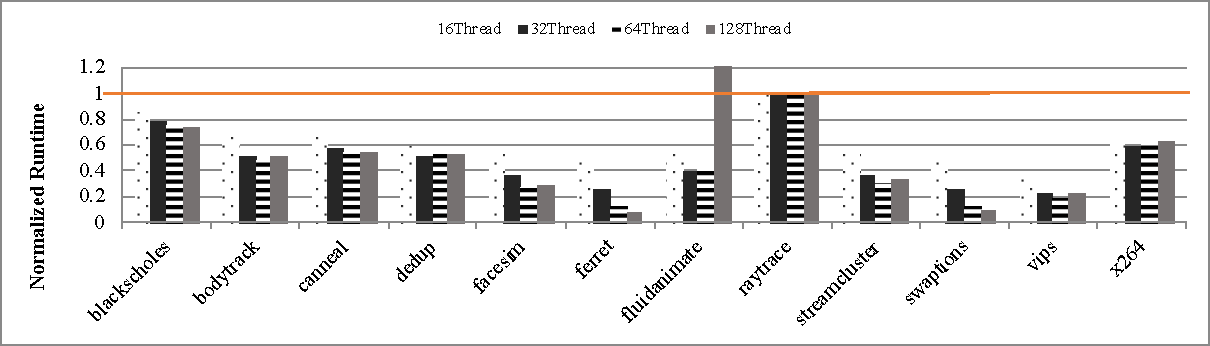
\includegraphics[width=5.5in]{figure/scalobility-pthread.pdf}
    \caption{Normalized performance of Linux's default allocator without binding for PARSEC benchmarks in Machine B}
    \label{pthread-scalibity}
\end{figure}

We will evaluate the scalability on 8threads, 16threads, 32 threads, 64 threads and 128 threads. 
(one node, two node, four nodes, and 8 nodes). 
	
\end{comment}


\subsection{Design Choices}
\label{sec:design}

This section further confirms \NM{}'s multiple design choices.
% all results shown in this section are normalized to the data of the default Linux allocator.  

%Based on our analysis, there are two reasons for this performance speedup. First, a thread will not be migrated to a different core, avoiding unnecessary remote accesses caused by cross-node migration, as further discussed in Section~\ref{sec:intro}. Second, \NM{}'s thread binding balances the workload, thus reducing the congestion of interconnect or one memory controller.
\subsubsection{Choices of Thread Binding}
\label{sec: threadbinding}

% \begin{figure*}[!h]
%     \centering
%     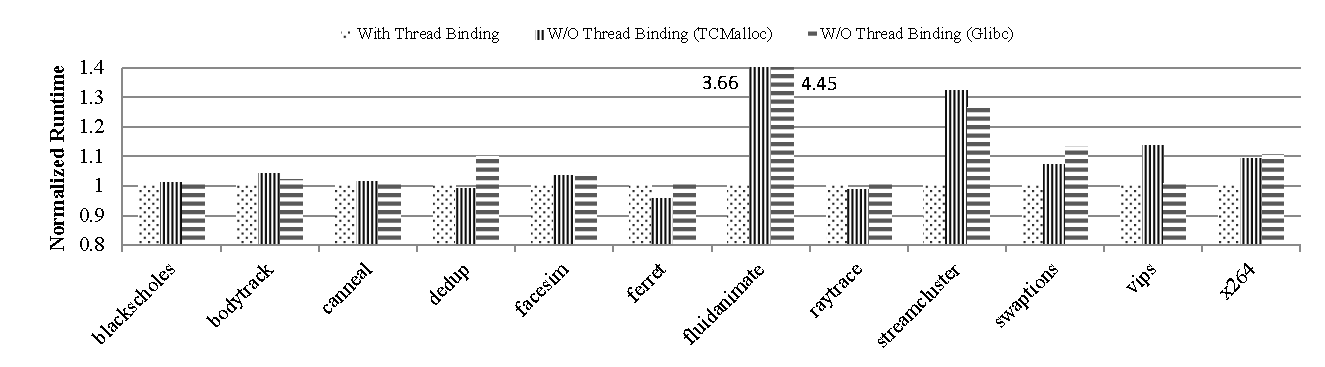
\includegraphics[width=6in]{figure/WO-pthread-binding3.pdf}
%     \caption{Normalized runtime with and without node-balanced thread binding for Glibc and TCMalloc.} 
%     \label{binding-pthread-scalibity}
% \end{figure*}

% \begin{figure*}[!ht]
%     \centering
%     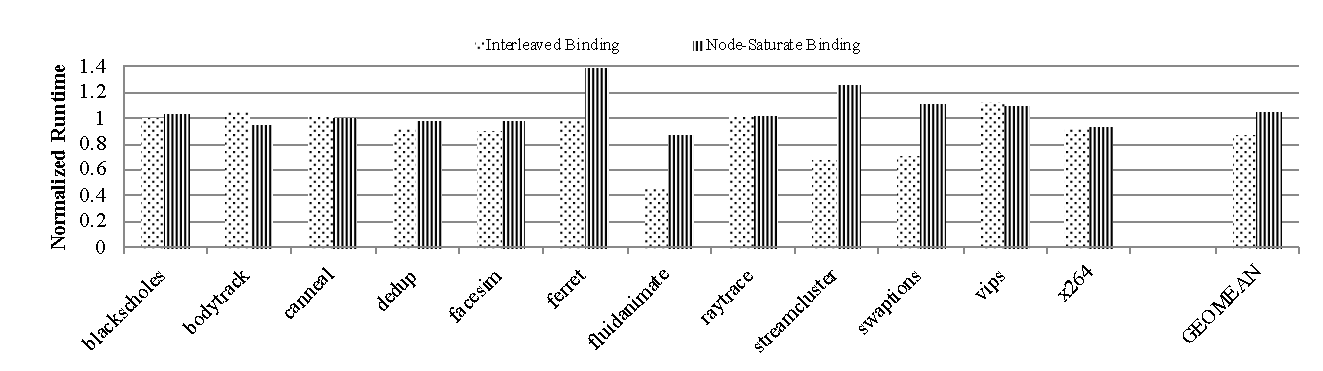
\includegraphics[width=5.5in]{figure/binding-policy.pdf}
%     \caption{ Node-Interleaved vs. Node-Saturate binding for Glibc, where results are normalized to those without binding.}
%     \label{fig:binding-policy}  
% \end{figure*}

\NEW{\NM{}'s memory management is based on binding, including thread binding and memory binding. We believe such bindings benefit the performance and open up other design opportunities, such as origin-aware memory management, metadata allocation and incremental sharing. The combination of all design choices makes \NM{} a faster and more efficient allocator. Therefore, we cannot evaluate the impact of thread binding by directly disabling it on \NM{} since other designs depend on it. To overcome this problem, we implement a thread binding library that allows other allocators to enable binding.}
Fig.\ref{binding-pthread-scalibity}(a) shows the \NEW{impact of thread binding on} two allocators, Glibc and TCMalloc.
% Fig.\ref{binding-pthread-scalibity}(a) shows the performance difference without thread binding for two allocators, Glibc and TCMalloc.
The results are normalized to the data with thread binding of each allocator, respectively, \NEW{so we omit the ones with thread binding. Thus, this figure can be considered to show how much slower it would run without thread binding.}
% We cannot evaluate \NM{} directly, since its mechanisms are tightened to thread binding, such as incremental sharing, origin-aware memory management and metadata allocation. 
Here we use the node-interleaved binding. As shown in Fig.\ref{binding-pthread-scalibity}(a), the thread binding improves the performance significantly for some applications. For instance, \texttt{fluidanimate} runs around $4.45\times$ faster on Glibc and $3.66\times$ faster on TCMalloc with the node-balanced thread binding. Similarly, \texttt{streamcluster} runs around 20\% and 30\% faster than the corresponding one without the binding. 
\NEW{We further use \texttt{perf}~\cite{perfweb} to analyze the reasons for the significant performance improvement of these two applications. The results confirm that remote accesses are significantly reduced with thread binding, mainly due to the elimination of thread migration. Interestingly, the cache miss rate also decreases with thread binding. Overall, thread binding will benefit the performance of most applications without hurting others,} 
% This clearly indicates that the thread binding will benefit the performance overall
which should be included in the memory allocator by default. 

% In particular, threads are bound to different nodes in a round-bin way, called node-balanced binding, which is the same as \NM{}.

We also compare two types of thread binding: node-interleaved or node-saturate thread binding. In node-saturate binding, we bind the maximum possible number of threads (same as the number of cores) to a node and then switch to the next node. As shown in Fig.\ref{binding-pthread-scalibity}(b), the node-interleaved thread binding is almost always better than node-saturate thread binding, except for \texttt{bodytrack}. On average, node-interleaved binding is around 19\% faster than node-saturate one for these evaluated applications. This indicates that people should use node-interleaved binding, if they would like to employ all hardware cores. However, if they only want to use partial cores, then the node-saturate binding could be a better choice. \NM{} allows users to adjust the binding option based on their needs.

% , proving the effectiveness of Node-Balanced thread binding.

\subsubsection{Impact of Transparent Huge Pages}

As discussed in \ref{sec:hugepages}, it's beneficial to embrace the transparent huge page support in modern systems. We evaluate the performance impact of transparent huge pages. The results are shown in Fig.~\ref{fig:hugepage}. When integrating with transparent huge pages, \NM{} achieves significantly better performance for \texttt{vips}, where it is running 16\% faster. On average, transparent huge pages improve the performance by about 2.62\%. There are no applications that run slower with huge pages. This clearly indicates that it is beneficial to enable transparent huge pages for the NUMA architecture, especially when \NM{} is used. 
Although \NM{} may increase its memory overhead from 2\% to 10\% when using huge pages, as shown in Table~\ref{tab:memory_consumption}, the memory overhead is still acceptable, given the hardware trend of increasing memory capacity.  


\subsubsection{Impact of Interleaved Heap} 
\label{sec:interleavedheap}

We also evaluate the potential benefit of the interleaved heap. The performance data is shown in Fig.\ref{fig:interleavedheap}. 
% Note that we have evaluated all PARSEC applications listed in Section~\ref{sec:performance}.
Based on the figure, we have the following conclusion: the interleaved heap will benefit (or at least has no harmful impact on) the performance for most applications. In particular, it improves the performance significantly on \texttt{fluidanimate} and \texttt{streamcluster}.  However, applications having a large portion of time spent in the serial phase, such as \texttt{canneal} and \texttt{raytrace}, may hurt the performance with the interleaved heap support. These two applications share the same property that they have a larger portion of the first serial phase. With the interleaved heap, \NM{} allocates the memory from different nodes interleavedly for the serial phase, instead of from the local node (based on the default first-touch policy). That is, some private objects allocated in a remote node may introduce unnecessary performance overhead due to remote accesses. Currently, we do not know why swaptions has a large \NEW{negative} performance impact when the interleaved heap is employed, whose performance can change dramatically when adding one \NEW{meaningless code line (declaration and assignment of a \texttt{volatile} variable) or changing the compilation flags}. We will keep investigating this. 
%Further, upon each allocation, \NM{} checks the callstack to confirm whether an allocation is from a potentially shared heap, which also introduces some overhead. Therefore, the interleaved heap will be enabled by default, unless programmers know that it will not benefit the performance.

Programmers can choose to enable or disable interleaved heap based on the applications. A simple metric is to use the portion of the serial phase inside multithreaded applications. For applications that are mostly running in the serial phase, turning off the interleaved heap support may be a better choice. That is, the interleaved heap will harm the serial execution, but may benefit the parallel execution because of its load balance. It is easy to turn on/off the interleaved heap via a compilation flag or the environment variable.  

\subsubsection{Impact of Origin-aware Deallocation}

\NM{} adopts an origin-aware deallocation that always returns the object to its original thread's or node's heap. We further verified the effect of this design and the results show that \NM{} runs 1.7\% slower if we do not consider the origin of freed objects. The details are omitted due to the space limitation. 

% \todo{other design choices: THP's impact on performance, origin-based deallocation, autonuma's impact...}

%, except applications with a large portion of serial phase (e.g., \texttt{canneal} and \texttt{raytrace})

%The interleaved heap could be utilized to avoid load imbalance issue for shared objets. 

%However, there are two issues for the interleaved heap. First, the allocator may not know whether an object is shared or not at the first time. Therefore, all objects that are allocated in the main heap (before creating any child thread) will be treated as the shared heap. Second, some applications are spending too much time in the serial phase, where the interleaved heap cannot benefit the performance for the serial phase. 





%figure ~\ref{parsec-no-interleaved-perf} we show some performance results of some applications that got significant different values after we shut down interleaved heap for \NM{}. We can see that for some applicatios with less data sharing between threads like ratrace and canneal, \NM{} could got significant improvements due to its low overheads and proper memory management. But for some other applications with intensive memory operations and sharing like fluidanimate, shutting down interleaved heap could hurt performance, since interleaved heap could help to distributed resource contention evenly over multi-nodes and then got low overheads.

%\subsubsection{Selective Huge Pages} 
%\label{sec:hugepage}

%Since the machine utilizes transparent huge pages by default, we evaluate the performance impact of huge page support on another machine with 2 NUMA-node, without enabling the transparent huge pages.
% A, the 2-node machine. We only utilize PARSEC applications for this evaluation. 

%\begin{figure}[!h]
%    \centering
%    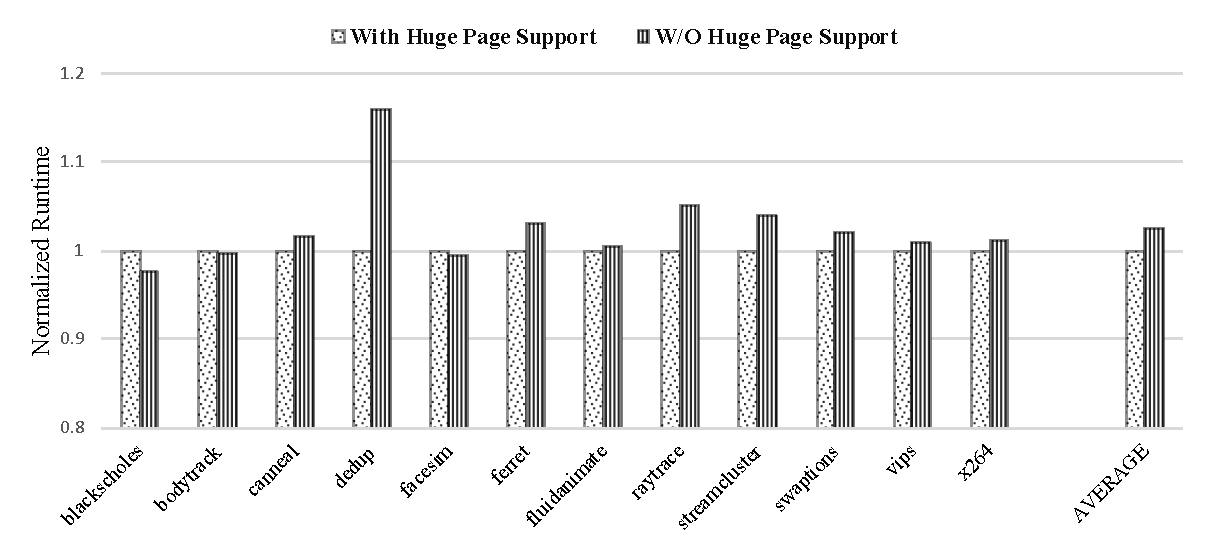
\includegraphics[width=3.2in]{figure/hugepage.pdf}
%    \caption{Normalized runtime with and without selective huge pages.}
%    \label{fig:hugepage}
%\end{figure}

%The results are shown in Figure~\ref{fig:hugepage}. When integrating with selective huge pages, \NM{} achieves a significantly better performance for \texttt{dedup}, where the performance difference is around 15\%. On average, the selective huge pages improves the performance of all evaluated applications about 2.5\%, and will not hurt the performance. This clearly indicates that it is beneficial to have selective huge pages for the NUMA architecture, especially given the fact of increasing memory size of hardware trend.  



\section{Related Work}

\paragraph{General Purpose Allocators:}

\paragraph{NUMA-aware Allocators:} 

\todo{All of the following papers are not read carefully. Most sentences are copied from the abstract}
Ogasawara proposes a NUMA-aware memory allocation for Java virtual machine~\cite{Ogasawara:2009:NMM:1640089.1640117}. The basic idea is to identify the Dominant Thread (DoT) via thread stack, synchronization information, and object reference graph.  

~\cite{wagle2015numa} focuses on the specific scenario, which is in-memory databases. 

~\cite{1419934}
Kaminski et al. proposes to make TCMalloc NUMA-aware~\cite{tcmallocnew}, with the very minimum effort. The idea is to maximize the local memory allocation with the node-based free list and page heap. However, this mechanism assumes that the memory deallocation from the current node will be always allocated from the local node. This is unfortunately not true for many cases, such as a producer-consumer model. Also, this allocator does not take advantage of 

~\cite{Majo:2011:MMN:1993478.1993481} :
Observation: it should take both data locality and cache contention into account to achieve good performance, and memory management cannot be decoupled from process scheduling. 
We describe two scheduling algorithms: maximum-local, which optimizes for maximum data locality, and its extension, N-MASS, which reduces data locality to avoid the performance degradation caused by cache contention. N-MASS is fine-tuned to support memory management on NUMA-multicores and improves performance up to 32\%, and 7\% on average, over the default setup in current Linux implementations.

% http://memkind.github.io/memkind/ 
% Use this to compare the performance difference
% However, this will require the change of applications to use their library. 
~\cite{cantalupo2015memkind} proposes a new library that allows users to manage their memory in very fine-granularity. However, they are not targeting for a general purpose allocator, which requires programmers to manage the memory explicitly. Unfortunately, this place unacceptable burden to programmers. More importantly, the explicit management based on one existing topology may not work well for a different topology. 



\paragraph{Other NUMA-related Systems:} 

Memory system performance in a numa multicore multiprocessor

~\cite{Majo:2015:LPC:2688500.2688509} proposes TBB-NUMA, a system that mainly focuses on task scheduling on NUMA architecture to achieve better performance. \NM{} employs a similar mechanism as TBB-NUMA to manage threads explicitly, but without relying on the human hints. \NM{} also deals with the memory allocation that is not presented in TBB-NUMA. 

~\cite{6704666} shows that a set of simple algorithmic changes coupled with commonly available OS functionality suffice to eliminate data sharing and to regularize the memory access patterns for a subset of the PARSEC parallel benchmarks. These simple source-level changes result in performance improvements of up to 3.1X, but more importantly, they lead to a fairer and more accurate performance evaluation on NUMA-multicore systems. In the default
configuration, OSs (such as Linux) tend to change the thread-to-core mapping during the execution of programs, which result in large performance variations.

~\cite{Bui:2019:EPV:3302424.3303960} talks about the virtualization of NUMA.

~\cite{jemalloc} introduces a round-robin fashion for arena allocation, and all locks and buffers will be local to the associated arena. Similarly, \NM{} also takes the similar approach. 

Scalloc utilizes the same-sized spans in order to encourage memory reuses~\cite{Scalloc}, which is also the same for \NM{}. Salloc has another two contributions, a global backend developed by concurrent data structures, and a constant-time front which returns the spans to the backend. 

Bolosky et. al. propose a simple mechanism to improve the performance by replicating read-only pages to multiple processors, moving pages to the processor that written them, and placing pages to the global memory if they are written by multiple processes ~\cite{Bolosky:1989:SBE:74850.74854}. bl


{
\bibliographystyle{ACM-Reference-Format}
\bibliography{ref,emery,tongping}
}

\end{document}
he 